\documentclass[preprint,12pt,letterpaper]{elsarticle}
\usepackage[T1]{fontenc}
\usepackage{textcomp}
\usepackage{amsmath,amssymb}
\usepackage{newtxtext,newtxmath}
\usepackage{graphicx}
\usepackage{booktabs}
\usepackage{longtable}
\usepackage{array}
\usepackage[hidelinks]{hyperref}
\usepackage[labelfont=bf,labelsep=period]{caption}
\captionsetup[figure]{name=Fig.}
\usepackage[margin=0.820000in]{geometry}
\makeatletter
\let\openbox\@undefined
\makeatother
\usepackage{amsthm}
\theoremstyle{definition}
\newtheorem{definition}{Definition}
\newtheorem{protocol}{Protocol}
\theoremstyle{plain}
\newtheorem{fact}{Fact}
\newtheorem{proposition}{Proposition}
\newtheorem{corollary}{Corollary}
\renewcommand{\thesection}{\arabic{section}}
\renewcommand{\thesubsection}{\thesection.\arabic{subsection}}
\setlength{\emergencystretch}{2em}
\begin{document}

\begin{frontmatter}

\title{Optimality gaps do not certify commitment in freight operations: an order-equivalence identity, a lever mechanism, and a two-dimensional release test}

\begin{abstract}
\setlength{\parindent}{0pt}\setlength{\parskip}{0.45ex}
A plan from a solver or a language model arrives with an optimality gap: its distance from a bound on the best achievable value. Practice treats a small gap as a licence to release. We show it is not, separating what the certificate is, why commitment breaks it, and how large the failure is. On twenty booking books, adding three slack plans to a six-plan pool leaves conflict at 20 of 20 while the penalty rises from 0.7 to 17.2 points.

The gap is affine in the objective with non-zero slope for any finite, non-zero bound; its within-instance ordering therefore equals the objective's, and a tighter bound moves which plans pass a threshold, never which is selected.

A commitment is priced at planning and charged at execution. Where a pool spans commitment levels, both are monotone with opposite signs and the gap-minimal and safest plans are its extremes (Proposition 1); where it does not, any rule reading only the number is constant on objective-level sets (Proposition 2). The penalty is the exposure slope integrated over the pool's commitment spread (Corollary 1).

Across 198 cases the gap's pick differs from the safest plan in 6.7 \% of repair instances (95 \% CI 3.3--13.2) and 94.9--96.8 \% of commitment instances, against 65--83 \% chance. A second exposure quantile cuts false releases from 41.2 \% to 20.5 \% for the bunker family (Fisher $p$ = 0.0008) and from 49.2 \% to 30.8 \% for the slot family, against a 25 \% baseline.
\end{abstract}

\begin{keyword}
LLM-generated plans \sep verification certificates \sep commitment \sep slot allocation \sep bunker procurement \sep decision-focused evaluation
\end{keyword}

\end{frontmatter}

\section{Introduction}

\subsection{The release decision}

Language-model planners have moved from advising to emitting the operational artefact: which bookings to accept, which ports to bunker at, which timetable to publish. Once the artefact is emitted it must be \textit{released} --- signed, sent to the customer, loaded --- and a release decision needs evidence. The evidence most pipelines already have is the number the solver printed alongside the plan: the optimality gap, the distance between the plan's objective value and a bound on the best achievable value (Definition 1).

That number is not incidental to practice; it is the default output of the toolchain. Most commercial MILP solvers terminate on a relative gap and print it in the log, so a plan arrives with a gap attached whether or not anyone asked for one. Procurement and tender documents in freight and bunkering commonly specify a tolerance of the form "within \textit{x} \% of optimal". Evaluation studies of language models as optimisers report distance to the optimum as the headline metric [1]. The working assumption --- usually implicit, occasionally written into a screening rule ("accept plans with a gap under 5 \%") --- is that a small gap means not only that the plan is close to the best plan the model admits, but that it is \textit{safe}: that it will still be executable after the uncertain parameters move.

\subsection{The question}

Is that assumption true? Specifically: under commitment, where the plan is locked before the uncertain parameters realise and cannot be re-optimised, does the gap rank candidate plans by their realised exposure?

\subsection{The answer, in three parts}

\textit{First}, the certificate is not a measurement of the plan at all; it is a monotone re-indexing of the objective value, for any bound (Fact 1). The algebra is one line; what it implies for release practice is not. The identity is exactly the property the practice relies on, and it forecloses the two natural defences: using a tighter bound cannot help, because every bound yields the same ordering, and switching to the absolute gap cannot help, because the absolute gap is affine in the objective too.

\textit{Second}, the failure under commitment is structural, not statistical. A commitment decision is priced twice: the planning objective pays for the volume promised at planning prices, and the realised exposure charges for the same volume at execution prices under drift. When both are monotone in committed volume with opposite signs --- the modal case in every commitment family we study --- their minimisers are the two opposite extremes of the candidate pool, so the gap-minimal plan is not merely sometimes risky, it is the riskiest plan available (Proposition 1). When the pool does not span commitment levels the theorem does not apply, and a weaker argument takes over: any release rule that reads only the reported number is constant on objective-level sets, so it cannot separate two plans that share an objective value and differ in exposure (Proposition 2).

\textit{Third}, the magnitude is governed by geometry, and this is the part that changes how the result should be used. The penalty is the exposure slope integrated over the pool's commitment spread (Corollary 1). It is therefore large where the pool spans commitment levels and negligible where the pool is concentrated at one level. That is not a caveat appended to the result; it is the result, and it is testable as a manipulation. We test it (\S 5.4): holding books, plans and drift draws fixed and adding three deliberate-slack plans to a six-plan pool, the top-1 conflict rate is unchanged at 20 of 20 books while the exposure penalty rises from 0.7 to 17.2 percentage points.

\subsection{Contributions}

\begin{enumerate}
\item \textbf{An identification fact, stated as such.} The gap is an affine function of the objective with a non-zero slope, for every bound; no gap-type certificate carries information beyond the objective's ordering (Fact 1, \S 3.1). The consequence for practice is sharper than the fact: threshold \textit{calibration} is bound-dependent and does not transfer between families (the same 5 \% rule admits 1.4 \% of slot candidates and 75.6 \% of bunker candidates), while the \textit{ordering} is bound-invariant. A gap threshold is a statement about the bound, not about the plan.
\item \textbf{An analytic mechanism with an explicit premise, and a magnitude law.} Proposition 1 derives the conflict from the two margins at which a commitment is priced, rather than measuring an association. Corollary 1 turns it into a quantitative law: the penalty is the integral of the exposure slope over the spread of committed volume in the pool.
\item \textbf{A controlled test of that law.} The twenty-book experiment is a two-arm contrast of pool composition with everything else fixed: 0.7 pp of exposure penalty at zero spread, 17.2 pp at 13 \% spread, same conflict rate. This also corrects a replication of ours that contained deliberate-slack plans and therefore overstated the effect (\S 5.4); we report the correction rather than the original.
\item \textbf{Measurement at scale, with the scope condition stated.} 198 usable instances in four families, Wilson and bootstrap intervals, filtered and unfiltered rates, adverse/symmetric/favourable drift, LLM and heuristic pools, two generations of candidates. The conflict rate is 6.7 \% under repair and 94.9--96.8 \% under commitment; it survives mean-zero drift (87.5--90.0 \%), is confined to adverse drift for its economic content, and is reproduced by a heuristic generator whose gaps are systematically better than the LLM's (90.0 \%). A pool of plans the solver cannot separate still spans 3.15 pp of exposure against 0.09 pp of gap, so the failure is a property of the certificate's resolution and not of the planner (\S 5.8).
\item \textbf{A release rule and its price.} A two-dimensional test --- gap quantile \textit{and} exposure quantile --- cuts the false-release rate from 49.2 \% to 30.8 \% in the slot family and from 41.2 \% to 20.5 \% in the bunker family, against the 25 \% a random release gives, at the cost of releasing 12--22 \% of the pool rather than 55 \%, and we price the alternative remedies: budgeted robustness, sample-average approximation and lift hedging all reduce exposure, at a gap cost we report in the metric's own units and, for the bunker family, in US dollars per voyage.
\end{enumerate}

\subsection{What this paper does not claim}

We do not claim that language models report their own gaps; the prompt never asks for one, and the certificate is attached by the pipeline (\S 2.1). We do not claim that the gap is a bad stopping criterion for a solver; it is the standard one and we use it as such. We do not claim a population effect from forty synthetic instances per maritime family, nor that the conflict is large in every deployment: \S 5.4 shows it is small when the candidate pool is concentrated, and we give the quantity that predicts its size. We do not claim that a strong planner would be immune. We test the obvious defence --- that a good planner narrows the pool until the plans are indistinguishable --- and it fails in the direction that matters: \S 5.8 builds pools of plans the solver cannot separate and finds a gap spread of 0.09 pp against an exposure spread of 3.15 pp. Tightness does not supply the immunity a strong planner would need, because the resolution of the certificate is what tightness consumes.

\section{Setting}

\subsection{Plans, certificates, and the release decision}

An instance $\omega$ defines a feasible set $\mathcal{X}(\omega)$ and an objective $f(\cdot; \omega)$. A planner --- a solver, a heuristic, or a language model --- emits a candidate set $X \subseteq \mathcal{X}(\omega)$, the plans generated during one planning cycle, and a \textbf{release rule} $A: X \to {accept, reject}$ decides which may be committed.

A \textbf{certificate} is any scalar $g: X \to \mathbb{R}$ attached to a plan as evidence of quality. Throughout, $f$ is written in the orientation the planner uses, and we let $F = -f$ when the planner minimises, so that $F$ is always "higher is better". Let $B_{F}$ be a bound on $\max F$ with $B_{F} \ge \max _{x\in \mathcal{X}} F(x)$.

\begin{definition}[gap-type certificate]
\begin{equation}
\tag{1}
g_{B}(x) = (B_{F} - F(x)) / |B_{F}|
\end{equation}

defined for $B_{F} \neq 0$
\end{definition}

Eq. (1) covers the variants in use. With $B_{F} = F*$ it is the gap to the exact optimum; with $B_{F}$ the LP relaxation, a Lagrangian bound [2], or the best bound at solver termination it is the gap a deployed solver prints; multiplying by $|B_{F}|$ gives the absolute gap; dividing by $|F*|$ instead of $|B_{F}|$ gives the conventional relative gap. All are affine in $F$.

Two regimes are distinguished throughout. Under \textbf{repair} a committed plan may be revised once the uncertain parameters realise, and the damage of a bad plan is bounded by its suboptimality. Under \textbf{commitment} the plan is locked at release and executed as written: there is no re-optimisation, so what matters is not the distance from optimal but the direction of the error and the volume over which it is taken.

\subsection{The commitment lever and realised exposure}

\begin{definition}[commitment lever]
For a plan $x$, $v(x) \ge 0$ is the volume of irreversible obligation it creates --- accepted TEU in slot allocation, contracted lift in bunker procurement.
\end{definition}

\begin{definition}[realised exposure]
For a drift model $\mathcal{D}$ over the instance parameters,

\begin{equation}
\tag{2}
R(x) = \mathbb{E}_{\omega'\sim \mathcal{D}}[ \ell(x, \omega') ]
\end{equation}

where $\ell$ is the realised shortfall of the committed plan executed as written, normalised by committed volume (slot overflow) or committed margin (budget overrun).
\end{definition}

The two maritime families instantiate Definitions 2 and 3 directly. In C, $v$ is committed TEU and $\ell$ is the share of committed volume that cannot be loaded on the binding leg after demand rises and capacity falls. In D, $v$ is lift contracted at the planning ports and $\ell$ is the budget overrun caused by buying the shortfall at a spot premium after prices rise and port caps fall.

\subsection{Four families}

Four families are used, two generic and two maritime. Table 1 fixes their vocabulary: what is committed, how drift moves the parameters, and how risk is realised.

\begin{table}[t]
\centering
\caption{Problem families, what is committed, and how risk is realised.}
\small
\setlength{\tabcolsep}{5pt}
\begin{tabular}{@{}>{\raggedright\arraybackslash}p{26.0pt}>{\raggedright\arraybackslash}p{102.0pt}>{\raggedright\arraybackslash}p{62.8pt}>{\raggedright\arraybackslash}p{74.4pt}>{\raggedright\arraybackslash}p{97.7pt}>{\raggedright\arraybackslash}p{71.1pt}@{}}
\toprule
ID & Problem & Decision & Committed & Adverse drift & Realised risk \\
\midrule
A & knapsack / diet / set-cover / combinatorial & choose a solution & nothing (repair allowed) & coefficient drift & cost regret \\
B & the same four classes & choose a solution & locked on submission & coefficient drift & 0/1 violation rate \\
C & liner slot allocation (multi-leg MCKP) & which bookings to accept & boxes and sailing & volume +10--20 \%, capacity $-$10--20 \% & rolled cargo (overflow) \\
D & bunker-port selection (Asia--Europe) & ports + lift volumes & freight and bunker clauses & price up, requirement up, port cap down & budget overrun \\
\bottomrule
\end{tabular}
\end{table}

Families A and B are the same instances and the same candidate solutions with only the regime changed: A has 143 instances and 614 candidates, all 143 appear unchanged in B, which adds 12 instances and 30 candidates. Nothing differs between them except whether the plan can be revised, which makes the A--B contrast the cleanest available design for the regime question. C and D are maritime, and they are the families in which the commitment lever is the decision variable rather than a by-product.

\section{Theory}

\subsection{What the certificate is: order equivalence}

\begin{fact}[order equivalence]
For any bound $B_{F}$ and any two candidates $x, y \in X$:

\begin{equation}
\tag{3}
g_{B}(x) < g_{B}(y) \iff F(x) > F(y)
\end{equation}

Every gap-type certificate is an affine function of $F$ with non-zero slope, and therefore induces the same weak order on $X$ as $F$ itself.
\end{fact}

\begin{proof}
Eq. (1) can be written $g_{B}(x) = 1 - F(x)/|B_{F}|$, an affine function of $F$ with slope $-1/|B_{F}| \neq 0$ for $B_{F}$ finite and non-zero. A strictly decreasing function reverses the total preorder induced by $F$, which is the relation displayed in Eq. (3). The absolute gap multiplies by the positive constant $|B_{F}|$; the relative gap replaces $B_{F}$ by \texttt{F*}, which changes the slope and intercept but not its sign.
\end{proof}

This is an identity, not a theorem, and we present it as such. It is stated because three defences of current practice depend on denying it, and each is closed by the same line of algebra. \textit{Use the true dual bound}: the ordering is identical for every bound, so the defence cannot change which plan is released. \textit{Use the absolute gap}: the absolute gap is the relative gap times a positive constant. \textit{Use more decimals}: no re-scaling of a monotone transform creates information.

Two consequences are worth separating, because they are routinely conflated:

\begin{enumerate}
\item \textbf{The ordering is bound-invariant; the calibration is not.} Which plan a gap selects does not depend on $B_{F}$; which plans pass a \textit{threshold} very much does, because a threshold is a statement about the scale of the bound. \S 5.2 measures both: $\rho = 1.000$ between the certificate computed against the exact optimum and against the solver's termination bound, with the selected plan identical in 100 \% of instances, while a 5 \% threshold admits 75.6 \% of bunker candidates against one bound and 69.0 \% against the other, and 1.4 \% of slot candidates against a bound of comparable tightness. A numeric threshold does not transfer between problem families, and practitioners who carry one across families are carrying a number whose meaning is bound- and family-specific.
\item \textbf{Order equivalence is not a defence of the metric.} The fact says the gap is a faithful re-expression of $f$. The question of this paper is whether $f$'s ordering is a risk ordering, and the answer is no under commitment. The fact matters because it removes the escape route: no re-engineering of the certificate, short of adding a variable, escapes the ordering of $f$.
\end{enumerate}

\subsection{Why it fails: the two margins of a commitment}

Write a plan as a portfolio of commitments. Two prices apply to the same portfolio.

At the \textbf{planning margin}, the objective is (to first order) linear in the commitments at planning prices, where $c_{i}$ is the commitment in dimension $i$ and $m_{i}$ the planning unit margin:

\begin{equation}
\tag{4}
F(x) = \Sigma_{i} m_{i} c_{i}(x)
\end{equation}

The planning objective is monotone in the commitments; whether the sign is positive (revenue) or negative (cost) is a property of the family, and it is the sign we carry through the propositions rather than assume.

At the \textbf{execution margin}, the exposure is the expected liability of honouring those commitments under drift, with $\ell$ the positive part of a constraint violation, hence convex and monotone in the commitments on the region where drift can bind:

\begin{equation}
\tag{5}
R(x) = \mathbb{E}[\ell(c(x), \xi)]
\end{equation}

Its direction is not assumed either --- it rises with promised volume in the capacity families and falls with coverage in the price family --- and that is exactly why the two margins can oppose with either sign. The two margins price the \textit{same} decision variable: a plan is paid for promising one way (Eq. (4)) and charged for having promised the other (Eq. (5)).

\begin{proposition}[lever opposition $\Rightarrow$ forced conflict]
Let $X$ be a candidate pool and suppose that on $X$

(P1) $g$ is strictly monotone in $v$ with sign $s_{g}$, and

(P2) $R$ is strictly monotone in $v$ with sign $s_{R}$, and

(P3) $s_{g} s_{R} = -1$.

Then the gap-minimal and the exposure-minimal plans are the two opposite extremes of $X$ in commitment, so the top-1 conflict indicator is 1, and the excess exposure of the gap-minimal plan equals the full range of exposure over $X$.
\end{proposition}

\begin{proof}
By Fact 1, $g$ is a strictly decreasing function of $F$, so (P1) makes $F$ strictly monotone in $v$ with sign $-s_{g}$; hence $\operatorname{argmin} g$ is $v_{max}$ if $s_{g} < 0$ and $v_{min}$ otherwise. By (P2)--(P3), $R$ is strictly monotone in $v$ with the opposite sign, so its minimiser is the other extreme. Strict monotonicity makes both minimisers unique, hence distinct, hence conflict. The excess equals $|R(v_{max}) - R(v_{min})|$ by strict monotonicity.
\end{proof}

The proposition is deliberately narrow in its hypotheses and strong in its conclusion: it does not require the lever to be the \textit{only} source of variation, only that it dominate the within-pool ordering of both functionals. What it does not do is predict how often (P1)--(P3) hold; \S 3.5 confronts that.

The premise has economic content and it holds for a reason in each family, with the sign of the opposition determined by which margin dominates:

\begin{itemize}
\item \textbf{Capacity-type commitment (A-locked, B, C).} The planning margin pays for accepted volume and the execution margin charges for it: commitment earns revenue per TEU and creates overflow when capacity falls. Then $s_{g} < 0$ (more commitment, smaller gap) and $s_{R} > 0$ (more commitment, more overflow). The gap's pick is the plan that promised the most. In C the rank correlation between the gap and committed TEU is $-1.000$ in the median instance --- the gap is, in that family, almost literally a measure of how much has been promised.
\item \textbf{Price-type commitment (D).} The planning objective is a cost, so the gap is normalised by committed cost and the sign of the opposition reverses. Lift contracted at the cheap port lowers the executed cost but raises the committed cost base; covering the last tonne of requirement forces lifting at an expensive port. Then $s_{g} > 0$ (more coverage, larger gap) and $s_{R} < 0$ (more coverage, smaller overrun, because the spot premium is avoided and the denominator is larger). The gap's pick is the plan that promised the least, and it is again the most exposed.
\end{itemize}

The two signs are opposite across families and the conflict is not: this is why we report conflict rates and not correlations (\S 5.1).

\textbf{Why the premises hold rather than being assumed.} Take one commitment dimension $v$ and let the realised capacity be $\tilde{c}$ with distribution $H$. The planning margin is linear, $F(v) = m v$ with $m > 0$, so $g$ is strictly decreasing in $v$: premise (P1) with $s_{g} < 0$. The execution liability is the positive part of a shortfall, $R(v) = \kappa \mathbb{E}[(v - \tilde{c})^{+}]$, whose derivative is $R'(v) = \kappa \Pr (\tilde{c} < v) > 0$ --- the probability that capacity binds. That derivative is the option-style slope already used in Corollary 1, and it makes $R$ strictly increasing: premise (P2) with $s_{R} > 0$. Then (P3) holds, and it is strict wherever the binding event has positive probability, which is by construction the region where drift can bind (Eq. 5). The price family runs the same two lines with the signs reversed --- $F(v) = -p v$ gives $s_{g} > 0$, and $R(v) = \pi \mathbb{E}[(\tilde{b} - v)^{+}]$ gives $R'(v) = -\pi \Pr (\tilde{b} > v) < 0$. The premises are therefore consequences of two primitives, a linear planning price and a positive-part liability, and not additional assumptions. What \S 3.5 tests is whether the primitives degrade in the archived instances --- a heterogeneity check on the data, not a check on the theorem.

\subsection{How large it is: a magnitude law}

\begin{corollary}[magnitude law]
Under (P1)--(P3), write $v_{min}$, $v_{max}$ for the extremes of $v$ on $X$. Then

\begin{equation}
\tag{6}
R(x_{g}) - R(x_{R}) = \int_{v_{min}}^{v_{max}} |R'(v)| dv
\end{equation}

so the penalty is the exposure slope integrated over the pool's commitment spread. It vanishes as the spread vanishes and equals the full exposure range when the pool spans the commitment range.
\end{corollary}

\begin{proof}
Both minimisers are at the extremes by Proposition 1, and $R$ is monotone, so the difference is the total variation of $R$ over $[v_{min}, v_{max}]$, which is the integral of $|R'|$.
\end{proof}

Two operational readings follow, and they are the ones we test. First, a pool concentrated at a single commitment level cannot generate a lever-driven conflict however bad the certificate is --- by Eq. (6) the penalty is $O(spread)$, not $O(1)$. Second, the same planner can generate a large penalty or a small one depending only on how widely its candidates commit, which is why the effect size is a property of the pool and not of the model.

\textbf{Composition.} Eq. (6) is written for a pool that varies one dimension. Where plans also differ in composition --- which bookings, which ports --- the penalty is the variation of $R$ along the pool's path in the lever, and is bounded above by the total variation of $R$ over the pool; the bound is attained when the pool is one-dimensional in $v$. \S 5.4 reading 4 is the case where composition carries a residual penalty with no spread at all, and it is small precisely because the composition axis moves $R$ little; \S 5.8 takes the opposite extreme, a pool with no spread in either direction, and measures what the certificate can still resolve there. We therefore use Eq. (6) as a directional law and verify it as a manipulation (\S 5.4) rather than as an equality.

\subsection{What no certificate-only rule can do}

Proposition 1 needs the pool to span commitment levels. The residual failure does not.

\begin{proposition}[level-set invisibility]
Let $A$ be any \textit{singleton} release rule --- one that returns a single plan as the released plan --- whose choice depends only on \texttt{g(x)} and on instance-level constants (thresholds, quantiles, $B_{F}$). Then $A$ is constant on every level set $\{x \in X : F(x) = c\}$. If two members of a level set differ in realised exposure, $A$ cannot separate them, and no re-parameterisation of $A$ can, because its inputs are equal on that set. Consequently the top-1 conflict rate is an exact measure of the best achievable performance of the class, not of a badly tuned member of it.
\end{proposition}

\begin{proof}
By Fact 1, $g$ is a strictly monotone function of $F$, so $g(x) = g(y)$ whenever $F(x) = F(y)$; a rule reading only $g$ and instance constants therefore assigns the same decision to $x$ and $y$. If $R(x) \neq R(y)$, at least one of the two decisions is wrong for one of them, and no change of parameters alters the equality of inputs.
\end{proof}

\textbf{Why the singleton restriction matters.} An earlier statement of this result in our own work applied it to subset rules, and that was wrong: a rule that releases a \textit{set} of plans is not a ranking, and level-set invisibility does not by itself make it fail, because releasing both members of a level set is a coherent (if uninformative) decision. The correct statement for subset rules is weaker and, for a release test, more useful: the released set is a union of level sets, so the worst exposure it admits is at least the worst exposure of the lowest-gap level set it contains, and no rule reading only the reported number can bound that quantity. A release \textit{test} therefore needs a second input; a release \textit{ranking} cannot be fixed at all. \S 5.6 builds the test.

\textbf{What Proposition 2 does not say.} It does not say that no rule can rank risk: a rule that reads an exposure estimate can, and Protocol 1 is one. It says the class of rules reading the reported number is exhausted --- tuning a threshold, switching normalisation, tightening the bound, reporting more decimals are all moves inside the class, and inside the class the failure measure is fixed by the data.

\subsection{The scope of the theory, stated plainly}

Proposition 1 is a sufficient condition, and its premise is not universal. In the LLM pools, the strong form of the premise --- the $v$-maximal plan attaining the minimal gap \textit{and} the $v$-minimal plan attaining the minimal risk --- holds in 50.0 \% of slot instances and 13.2 \% of bunker instances. The weaker sign-opposition form holds in 91.7 \% and 86.8 \%. Neither number explains a conflict rate of 95 \%.

We therefore make no claim that the theory predicts the rate. What it delivers is directional and quantitative in a different sense:

\begin{enumerate}
\item \textbf{The direction is not an empirical regularity.} Conditional on the premise, conflict is certain and the identity of the two picks is determined by the sign of the opposition (Proposition 1). A referee who is unmoved by a correlation should be moved by this, because the alternative hypothesis --- that the gap and the exposure order plans similarly under commitment --- is incompatible with the structure of a commitment problem rather than merely unlikely in our sample.
\item \textbf{The magnitude is predicted by a measurable pool statistic.} Corollary 1 says the penalty scales with the spread of committed volume and with the slope of exposure in it. That is a falsifiable statement about \textit{between-pool} differences, and \S 5.4 tests it with a manipulation in which nothing but the spread changes.
\item \textbf{The residual rate has a second, unconditional mechanism.} Where the premise fails, exposure still varies within objective-level sets, and Proposition 2 says no gap-only rule can see that variation. The union of the two arguments covers the data; neither alone does, and we say so instead of choosing the flattering one.
\end{enumerate}

A controlled stress test makes the same point numerically, and it also tells a practitioner what to expect in a new problem. With synthetic pools built as $g = 0.55 - 0.35 v + \sigma \xi$ and $R = 0.12 + 0.30 v + \sigma \xi'$ (400 pools per level, 4--7 candidates each), the conflict rate is 1.000 at $\sigma = 0$, 0.995 at $\sigma = 0.05$, 0.925 at $\sigma = 0.10$, 0.857 at $\sigma = 0.20$ and 0.840 at $\sigma = 0.30$. The observed 94.9--96.8 \% corresponds to $\sigma \approx 0.07\text{--}0.08$ of additive heterogeneity: our candidate pools are mostly, not purely, lever-driven. The conflict approaches totality insofar as commitment volume is the dominant degree of freedom in the pool --- which is a statement about the pool, and one an operator can check before trusting or distrusting a certificate.

\section{Protocol}

\subsection{Candidates}

\textbf{C and D use genuine LLM candidates} from local open-weight models (\texttt{qwen2.5:7b}, \texttt{mistral:7b}) at temperatures 0.4, 0.7 and 1.0, JSON-constrained decoding, one sample per model--temperature pair per instance, duplicates removed. Heuristic candidate sets are generated in parallel and used as a generator-robustness check (\S 5.4), never as a substitute for the LLM pools in the headline numbers.

\begin{itemize}
\item \textbf{C.} 40 instances of a 4-leg service with 18--24 booking requests and a demand/capacity ratio of 1.05--1.30. 214 recorded calls produced 163 capacity-feasible candidates (76 \%); the 51 infeasible plans are not executable and are excluded. Median gap of retained candidates is 0.52 --- these are untuned 7B models, not strong planners, and \S 5.4 and \S 7 treat that squarely.
\item \textbf{D.} 40 instances with six candidate bunker ports (Singapore, Fujairah, Port Klang, Colombo, Suez, Rotterdam), 2024-magnitude VLSFO prices (588--660 USD/t), per-port lift caps and deviation costs. 179 calls produced 179 parses; 91 (51 \%) meet the voyage requirement nominally. Because the vessel must sail, shortfalls are bought at a 1.5$\times$ spot premium and charged to execution cost. This is not a favour to the evaluation: it is the consequence of under-lifting under commitment, and it is why the D results have a dollar interpretation.
\end{itemize}

\subsection{Risk definitions}

\begin{itemize}
\item \textbf{A (repair):} cost regret $(C_{repaired} - C_{clairvoyant})/|C_{clairvoyant}|$.
\item \textbf{B (commitment):} indicator that at least one constraint is violated after drift.
\item \textbf{C (commitment):} $overflow = \max _{k} (load_{k} - cap_{k})^+ / \Sigma_{i} q_{i} x_{i}$, the share of committed volume that cannot be loaded on the binding leg.
\item \textbf{D (commitment):} $overrun = (C_{executed} - C_{committed})/|C_{committed}|$, also recorded in USD.
\end{itemize}

For every family we also compute the \textbf{absolute} counterpart, because a referee will ask whether the result is an artefact of the ratio denominator.

\subsection{Metrics}

\begin{itemize}
\item \textbf{Top-1 conflict rate} (primary): share of instances where $\operatorname{argmin} g \neq \operatorname{argmin} R$.
\item \textbf{Endpoint positions}: within-instance ranks in $[0,1]$; the gap rank of the safest plan, and the risk rank of the gap-optimal plan.
\item \textbf{Lever diagnostics}: $\rho(v, g)$, $\rho(v, R)$, the share of instances with opposed signs, the share with exact endpoint reversal, the $v$-position of each pick.
\item \textbf{Pass rate}: the mean over instances of the share of that instance's candidates whose gap is at most the stated threshold; the median of the same per-instance shares is reported alongside where the two differ.
\item \textbf{False release}: a plan is \textit{falsely released} if it is accepted by a rule and its true risk lies in the top quartile of its instance.
\end{itemize}

\subsection{Inference}

Every conflict rate is reported with a Wilson 95 \% interval and an instance-level bootstrap (2,000 resamples, percentile interval). Every effect size is a paired median over instances with a bootstrap interval of the same construction (5,000 resamples, fixed seed; \texttt{effect\_\allowbreak{}ci.\allowbreak{}csv}), so that one rule underlies every interval in the paper. We report both interval types because they disagree in the direction a referee should check: for B the Wilson interval is $[0.838, 0.994]$ and the bootstrap interval $[0.903, 1.000]$. Neither is used to claim a point estimate finer than the interval supports.

\subsection{The tie filter, and the unfiltered numbers}

An instance enters the primary metric only if at least three candidates exist and at least two differ in realised risk. Where every candidate carries identical risk, $\operatorname{argmin}$ is an arbitrary tie and the conflict indicator carries no information. The filter is mechanical, applied uniformly, and was fixed before the final numbers were computed --- but it is also \textit{consequential}, and hiding that would be the single easiest way to inflate the headline. It reduces B from 155 to 31 instances (46 have fewer than three candidates; 78 of the remaining 109 violate identically), C from 37 to 24, A from 143 to 104 and D from 40 to 39. Table 2 therefore carries the unfiltered column beside the filtered one. The unfiltered commitment rates are 69.0 \% (B), 86.5 \% (C) and 95.0 \% (D); the filtered ones are 96.8 \%, 95.8 \% and 94.9 \%. The qualitative claim survives either way; only its magnitude depends on the filter, and B is where the dependence is large.

\subsection{Drift direction and baselines}

Because a risk ordering can only be informative if drift can hurt, every maritime result is computed under three drift directions: \textit{adverse} (the shock moves parameters against the plan), \textit{symmetric} (mean-zero, equally likely either way) and \textit{favourable} (the shock helps). This is not a robustness check bolted on afterwards; it is the test of whether the conflict has economic content or is an artefact of a one-sided drift model (\S 5.4).

\textbf{The band, against a public series.} The band is an assumption, and the one channel that can be checked against public data has been. Daily Brent (\texttt{DCOILBRENTEU}, FRED, 2 January 2024 -- 27 October 2026, 715 observations) gives 691 overlapping 24-trading-day log returns --- the voyage of \S 5.7 is 24.1 days --- with a median absolute move of 6.5 \%, a 90th percentile of 24.0 \%, a 95th percentile of 32.2 \%, and 14.8 \% of windows beyond $\pm$20 \%. The band's average price move, +7.5 \%, is three times the empirical average of $\mathbb{E}[e^{r}] - 1 = +2.5 \%$, so in the body of the distribution the assumption is conservative; its 20 \% cap sits near the empirical 85th percentile, so in the tail it is thin. \S 5.7 substitutes the empirical distribution and reports both effects.

Four remedies are evaluated on the same adverse scenarios as the LLM pools, so that the comparison is at equal risk exposure: the nominal optimum; a Bertsimas--Sim budgeted-uncertainty counterpart at $\Gamma = 2.2$ and $\Gamma = 4.4$ (family C); a two-stage sample-average approximation (SAA) over 40 scenarios (family C); and lift hedging at the $q = 50, 75, 90, 95$ quantile of the requirement (family D). Gap and exposure are reported for each, and for D the committed cost base and the absolute exposure in USD, which is the denominator an operator would quote.

\subsection{Analysis plan}

Families, drift protocol, metrics, tie filter, interval methods and the stress design were fixed before the final numbers were computed. The certificate-swap experiment (\S 5.2), the effect-size analysis (\S 5.5), the alternative-lever analysis (\S 5.3), the release test (\S 5.6), the drift-direction and baseline analyses (\S 5.4--5.5) and the twenty-book manipulation (\S 5.4) were added in response to internal review; all are reported whether or not they support the main claim. The alternative-lever analysis in particular was designed to \textit{falsify} the mechanism, and its failure to do so is reported as such. The twenty-book manipulation replaces an earlier version of that experiment which contained deliberate-slack plans and therefore overstated the penalty; the corrected ensemble is the primary result and the original design is retained as the second arm of the manipulation.

\section{Results}

\subsection{The regime contrast}

\begin{table}[t]
\centering
\caption{Gap versus realised risk: filtered (and unfiltered) conflict rates with interval estimates.}
\scriptsize
\setlength{\tabcolsep}{3pt}
\begin{tabular}{@{}>{\raggedright\arraybackslash}p{47.5pt}>{\raggedright\arraybackslash}p{43.5pt}>{\raggedright\arraybackslash}p{19.9pt}>{\raggedright\arraybackslash}p{28.8pt}>{\raggedright\arraybackslash}p{57.8pt}>{\raggedright\arraybackslash}p{45.8pt}>{\raggedright\arraybackslash}p{40.3pt}>{\raggedright\arraybackslash}p{49.0pt}>{\raggedright\arraybackslash}p{46.8pt}>{\raggedright\arraybackslash}p{54.6pt}@{}}
\toprule
Family & Inst. (filtered / all) & $\rho$ ratio & $\rho$ absolute & Top-1 conflict, filtered & 95 \% CI (Wilson) & Bootstrap 95 \% & Conflict, unfiltered & Gap rank of safest & Risk rank of gap pick \\
\midrule
A repair $\cdot$ regret & 104 / 143 & \textbf{+1.000} & +1.000 & \textbf{6.7 \%} & [3.3, 13.2] & [2.9, 12.5] & 5.6 \% & 0.00 & 0.00 \\
B commit $\cdot$ violation & 31 / 155 & $-$0.617 & $-$0.617 & \textbf{96.8 \%} & [83.8, 99.4] & [90.3, 100.0] & 69.0 \% & 0.67 & 0.94 \\
C slots $\cdot$ overflow & 24 / 37 & $-$0.775 & $-$0.775 & \textbf{95.8 \%} & [79.8, 99.3] & [87.5, 100.0] & 86.5 \% & 1.00 & 1.00 \\
D bunker $\cdot$ overrun & 39 / 40 & $-$0.486 & $-$0.300 & \textbf{94.9 \%} & [83.1, 98.6] & [87.2, 100.0] & 95.0 \% & 1.00 & 0.75 \\
\bottomrule
\end{tabular}
\end{table}

\begin{itemize}
\item \textbf{The regime contrast is clean.} A and B are the same candidate sets. Replace "repair allowed" with "submitted = locked" and the conflict rate moves from 6.7 \% to 96.8 \%, and $\rho$ from +1.00 to $-$0.62. Under repair the gap \textit{is} a risk ordering: $\rho = +1.000$ exactly in 83.7 \% of the 104 usable instances, with a median of exactly 1.000. This is worth stating plainly, because it explains the practice --- the proxy works in the regime where the people who designed it were working, and a repair regime is what most solver pipelines are evaluated in.
\item \textbf{C: the gap-optimal plan is the worst plan.} Its median within-instance risk rank is 1.00 --- in the median instance it rolls more cargo than any other candidate --- and the safest plan's median gap rank is also 1.00. That is the median instance, not every instance: the two signs are opposed in 91.7 \% of pools and the two picks exchange the lever endpoints exactly in half of them (lever-endpoint reversal 0.50).
\item \textbf{D: safety has a price the gap refuses to pay.} The safest plan sits at the top of the gap distribution (median gap rank 1.00, median gap 0.533 against the gap pick's 0.0004); the gap's pick has median risk rank 0.75 and is the riskiest plan in 43.6 \% of instances.
\item \textbf{The correlation coefficient is not the finding.} $\rho$ changes sign between families and between normalisations (D: $-$0.486 ratio, $-$0.300 absolute); the conflict rate does not (D: 94.9 \% either way). Fig. 1(a) shows the sign instability and Fig. 1(b) the stable conflict rate; Fig. 1(c) shows the two minima at opposite ends, and Fig. 1(d) the mechanism.
\item \textbf{The conflict rate has a null, and it is not zero.} A pool of $n$ plans is ordered at random with probability $1 - 1/n$ of putting the gap's pick and the safest plan at the same end, so a rate near 100 \% has to be read against that, not against 0. The usable pools carry a median of four plans in C and three in D, giving mean chance levels of 75.1 \% and 64.9 \%; the six-plan book pools give 83.3 \%. The measured rates clear the null by 14 to 30 points, and the C and D Wilson intervals exclude it; the B interval's lower bound, 83.8 \%, clears the six-plan null by half a point. What separates the result from a random ordering is therefore not the rate but the pick: the gap's chosen plan carries median risk rank 0.75--1.00 and a penalty of 3.9--25.0 points, where a random ordering places it at 0.5 (\texttt{screen\_\allowbreak{}pairwise.\allowbreak{}py}).
\end{itemize}

\subsection{The certificate does not matter; the ordering does}

If Fact 1 is right, replacing the exact optimum with a genuine solver bound must leave every ranking untouched. We recompute the entire analysis for C and D against the MIP solver's own bound at termination; Table 3 reports the swap.

\begin{table}[t]
\centering
\caption{Certificate swap: exact optimum versus solver bound.}
\footnotesize
\setlength{\tabcolsep}{4pt}
\begin{tabular}{@{}>{\raggedright\arraybackslash}p{29.5pt}>{\raggedright\arraybackslash}p{71.8pt}>{\raggedright\arraybackslash}p{71.0pt}>{\raggedright\arraybackslash}p{40.6pt}>{\raggedright\arraybackslash}p{52.6pt}>{\raggedright\arraybackslash}p{91.9pt}>{\raggedright\arraybackslash}p{80.6pt}@{}}
\toprule
Family & Median bound/optimum & $\rho(gap_{true},\allowbreak{}gap_{bound})$ & Same argmin & Conflict (true $\to$ bound) & Pass rate at 5 \% (true $\to$ bound) & Median gap (true $\to$ bound) \\
\midrule
C slots & 1.016 & \textbf{1.000} & \textbf{100 \%} & 85.7 \% $\to$ 85.7 \% & 1.4 \% $\to$ 1.4 \% & 0.516 $\to$ 0.519 \\
D bunker & 0.990 & \textbf{1.000} & \textbf{100 \%} & 94.9 \% $\to$ 94.9 \% & \textbf{75.6 \% $\to$ 69.0 \%} & 0.020 $\to$ 0.031 \\
\bottomrule
\end{tabular}
\end{table}

Three things follow, and they are the empirical content of Fact 1.

\begin{enumerate}
\item \textbf{Ranking is invariant.} The Spearman correlation between the two certificates is 1.000 in both families and the selected plan is identical in 100 \% of instances. This is not an empirical regularity; the identity says it must be so. It is reported because a reader is entitled to see the identity do some work.
\item \textbf{The conflict rate is invariant, exactly.} 85.7 \% either way in C, 94.9 \% either way in D. The C sample here is the 35 instances carrying a usable candidate pair, not the 24-instance filtered sample of Table 2 (95.8 \%); the comparison that matters is true-versus-bound within one fixed sample. A referee who suspects the result is an artefact of using an exact optimum --- a gap that is "too clean" --- is answered: the same failure occurs with the bound a deployed solver would actually report.
\item \textbf{Calibration is not invariant, and this is the practitioner's problem.} The same 5 \% threshold admits 75.6 \% of D candidates against the exact optimum and 69.0 \% against the bound: 6.6 points of the admitted set move with no change in ranking. And the same threshold admits 1.4 \% in C and 75.6 \% in D --- a 54-fold difference in permissiveness for a rule that looks identical on paper. The C and D bound ratios bracket 1 (1.016 and 0.990), so this is not a test against a trivially tight bound: the D bound is valid but looser, and it is in D that the admitted set moves.
\end{enumerate}

\subsection{The mechanism}

\textbf{Lever diagnostics (LLM pools).} In C, $\rho(v, g) = -1.000$ and $\rho(v, R) = +0.773$ in the median instance; signs are opposed in 91.7 \% of the 24 instances and the endpoint reversal holds in 50.0 \%. The gap's pick sits at $v$-rank 1.00 and the safest plan at $v$-rank 0.00. In D, $\rho(v, g) = +0.775$ and $\rho(v, R) = -0.821$, opposed in 86.8 \% of 38 instances, endpoint reversal in 13.2 \%; the gap's pick sits at $v$-rank 0.23 and the safest at 1.00. Fig. 6 shows the trace behind these coefficients for the instance closest to each family's median, so that the ranks can be read as quantities: in C (instance 1001, $\rho = -0.77$) rolling more cargo lowers the gap and raises overflow at every step, and in D (instance 2038, $\rho = -0.49$) the same opposition runs along the lifted tonnes and the budget overrun. The signs are opposite between families because the price-type and capacity-type margins oppose in opposite directions (\S 3.2), and the conflict does not care: 95.8 \% and 94.7 \% (38 D instances carry a usable lever pair; on all 39 the rate is 94.9 \%). Corollary 1's premise is what these diagnostics measure, and its prediction --- that the penalty is the exposure range spanned by the pool --- is what \S 5.4 tests.

\textbf{Alternative levers (an attempt to falsify).} If the conflict were an artefact of our choice of $v$, replacing $v$ would dissolve it. It does not. In C, with 24 instances, the conflict is 95.8 \% whether the lever is committed TEU (opposed in 91.7 \%), revenue (87.5 \%), bookings accepted (87.5 \%) or peak utilisation (95.8 \%). In D, with 38 instances, it is 94.7 \% for lift coverage and for lift tonnes (86.8 \% opposed), 100 \% for ports called (23 instances, 100 \% opposed) and 94.9 \% for total cost (39 instances, 76.9 \% opposed). Any monotone re-expression of the commitment level carries the same conflict; the conflict is a property of the metric, not of the diagnostic. The lever is in any case not chosen post hoc: it is the decision variable of the model --- accepted bookings in C, contracted lift in D --- fixed before any risk is computed.

\textbf{Paired stratification.} If the conflict is lever-driven it should strengthen as the commitment gap between two candidates widens. Stratifying all candidate pairs by $|\Delta v|$ into terciles, the discordant-pair share rises monotonically: C 0.762 (n = 42) $\to$ 0.897 (n = 39) $\to$ 0.907 (n = 54); D 0.571 (n = 112) $\to$ 0.615 (n = 122) $\to$ 0.854 (n = 89). Pairs that differ little in commitment differ little in their verdicts. This is the sharpest within-pool evidence that the conflict is generated by the lever rather than by noise in the risk estimate.

\textbf{Generator robustness.} The conflict does not depend on who generated the candidates. Heuristic candidates in C give $\rho = +0.148$, the \textit{opposite} sign to the LLM candidates' $-$0.775, yet a conflict rate of 90.0 \% versus 95.8 \%. In D the heuristic pool gives $-$0.411 and 90.0 \% versus the LLM pool's $-$0.486 and 94.9 \%. The C heuristic pool is a much stronger planner than the LLM pool --- median gap 0.030 against 0.520, a factor of 17 --- while in D the two pools are comparable (0.025 against 0.019), so C also varies gap quality and not just generator identity. A pool with systematically better gaps and a different correlation structure produces the same failure, which is the strongest available evidence that the object of criticism is the metric and not the model. Regeneration moves almost nothing: local sampling is not bit-reproducible at fixed seed, so both families were regenerated from scratch and both generations archived; run-to-run spread is $\le$ 0.014 in $\rho$ and $\le$ 2.5 points in the conflict rate (C: 93.3 \% $\to$ 95.8 \% over 30 $\to$ 24 usable instances; D: 94.9 \% $\to$ 94.9 \%). The one quantity that did move materially --- the gap rank of the safest C plan, 0.78 $\to$ 1.00 --- is reported as a range rather than a point. The heuristic pools were generated twice as well, with the same generator and different seeds: C gives 90.0 \% at $\rho = +0.148$ in \texttt{unified\_\allowbreak{}robust.\allowbreak{}csv} and 87.5 \% at $\rho = +0.117$ in the drift arm of Table 4; D gives 90.0 \% at $\rho = -0.411$ and 90.0 \% at $\rho = -0.446$. Table 4 uses the second generation because it shares the drift protocol with the LLM rows.

Because $\rho$ can change sign under a generator swap, \textbf{we do not claim a correlation}. We claim an ordering conflict at the extremes, which Fact 1 and Proposition 2 say is the quantity that determines what a release rule can do.

\subsection{The lever-spread manipulation}

Corollary 1 makes a between-pool prediction: at fixed exposure slope, the penalty grows with the commitment spread of the pool and vanishes without it. We can test that prediction directly, because we can build two pools that differ in that one dimension and in nothing else.

Twenty booking books are generated on the real Asia--Europe rotation. Each book supplies six heuristic plans (two slot-ordering rules $\times$ three bunker strategies), all loaded to capacity; the six commit the same volume up to the rounding of the last accepted booking --- median spread 0 \%, and at most 2.3 \% in the nine books where it is non-zero (in the other eleven all six plans commit identical volume) --- since they accept bookings until the leg binds. The second arm adds three deliberate-slack plans at 95 \%, 90 \% and 80 \% of capacity, which span the commitment level by construction (median spread 13.2 \% of mean committed TEU); the six original plans are unchanged, the drift draws are identical, and the exposure functional is identical.

\begin{table}[t]
\centering
\caption{Conflict is universal, the penalty is a spread statistic.}
\scriptsize
\setlength{\tabcolsep}{3pt}
\begin{tabular}{@{}>{\raggedright\arraybackslash}p{107.9pt}>{\raggedright\arraybackslash}p{15.5pt}>{\raggedright\arraybackslash}p{91.7pt}>{\raggedright\arraybackslash}p{26.0pt}>{\raggedright\arraybackslash}p{23.7pt}>{\raggedright\arraybackslash}p{51.9pt}>{\raggedright\arraybackslash}p{48.5pt}>{\raggedright\arraybackslash}p{80.7pt}@{}}
\toprule
Pool (drift) & Inst. & Lever spread (CV of utilisation) & Conflict & $\rho_{med}$ & Exposure, gap pick & Exposure, safest & Penalty [95 \% CI] \\
\midrule
C $\cdot$ LLM (adverse) & 24 & 30.7 \% & 95.8 \% & $-$0.775 & 3.9 \% & 0.0 \% & \textbf{+3.9 pp} [2.2, 6.0] \\
C $\cdot$ heuristic (adverse) & 40 & 2.8 \% & 87.5 \% & +0.117 & 7.1 \% & 4.4 \% & +2.3 pp [1.8, 2.8] \\
C $\cdot$ heuristic (symmetric) & 40 & 2.8 \% & 87.5 \% & +0.165 & 1.8 \% & 0.6 \% & +0.8 pp [0.5, 1.0] \\
D $\cdot$ LLM (adverse) & 39 & 21.0 \% & 94.9 \% & $-$0.486 & 25.0 \% & 1.8 \% & \textbf{+21.7 pp} [6.3, 24.7] \\
D $\cdot$ heuristic (adverse) & 40 & 0 \% level, composition varies & 90.0 \% & $-$0.446 & 24.2 \% & 21.9 \% & +1.6 pp [1.0, 2.2] \\
D $\cdot$ heuristic (symmetric) & 40 & 0 \% & 90.0 \% & $-$0.133 & 7.0 \% & 4.1 \% & +2.3 pp [1.6, 2.9] \\
D $\cdot$ heuristic (favourable) & 40 & 0 \% & 85.0 \% & +0.086 & $-$7.1 \% & $-$7.9 \% & +0.8 pp [0.5, 1.0] (windfall) \\
Books, 6 full-capacity plans (adverse) & 20 & \textbf{0 \%} (max 2.3 \%) & \textbf{20 / 20} & +0.500 & 19.8 \% & 18.7 \% & \textbf{+0.7 pp} [0.6, 1.3] \\
Books, 6 + 3 slack plans (adverse) & 20 & \textbf{13.2 \%} & \textbf{20 / 20} & $-$0.179 & 19.8 \% & 2.5 \% & \textbf{+17.2 pp} [16.7, 17.4] \\
\bottomrule
\end{tabular}
\end{table}

\textit{Note.} Exposure cells are medians of per-instance values. The penalty cell is the paired statistic --- the median over instances of the exposure difference --- with a percentile bootstrap interval over instances (5,000 resamples, fixed seed; \texttt{effect\_\allowbreak{}ci.\allowbreak{}csv}). It need not equal the difference of the two exposure cells: in the full-capacity arm the difference of the medians is 1.1 points against a paired median of 0.66, because the sign of the per-book difference varies. All nine intervals exclude zero at 95 \%, and all nine do so under a Bonferroni correction for nine comparisons (99.4 \% intervals; \texttt{effect\_\allowbreak{}ci.\allowbreak{}csv}). Lever spread is the median within-instance coefficient of variation of the lever across the pool's candidates --- utilisation in C, tank fill in D --- computed on the instances in the row (\texttt{lever\_\allowbreak{}cv.\allowbreak{}csv}); for the two book rows the lever is committed TEU and the cell reports the relative range, (max $-$ min)/mean, over the six or nine plans (\texttt{rev2b\_\allowbreak{}books\_\allowbreak{}arms.\allowbreak{}csv}).

The last two rows are the experiment. Books, candidate generation, drift draws and the risk functional are identical; three plans that commit less volume are added, and pool size rises from six to nine, which this manipulation cannot avoid. The conflict indicator sits at its ceiling in both arms (20 of 20 under the adverse drift of these rows; under symmetric drift the six-plan arm shows conflict in only 16 of the 20 books) and therefore cannot discriminate, which is why the outcome variable is the penalty rather than the conflict rate: it rises from 0.66 to 17.16 percentage points, a 26-fold change, and the rank correlation between gap and exposure flips from +0.500 to $-$0.179. Fig. 2(a) plots the twenty paired differences.

Four readings, the first of which corrects our own earlier report.

\begin{enumerate}
\item \textbf{The original twenty-book result was partly a design artefact, and we say which part.} An earlier version of this ensemble was the slack-augmented arm alone, and it reported a large exposure gap as a replication of the mechanism --- 19.5 \% against 3.1 \% in that report, 19.8 \% against 2.5 \% when the same arm is re-run with the archived generator, which is the figure we quote everywhere else. The conflict did replicate --- 20 of 20 books --- but the \textit{economic} magnitude was manufactured by three plans per book that were built to commit less. The clean arm shows the conflict at 20 of 20 with a 0.7-point penalty. That conflict is a tie-level statement: the six plans commit the same volume to within one booking and differ only in \textit{which} bookings they accept, so the two metrics disagree about the ranking of near-equal plans while the exposure difference is two-thirds of a point. Both arms reproduce the ordering; only the second reproduces a penalty worth pricing. The correct statement is not that the operational ensemble reproduces a large penalty but that it reproduces the \textit{ordering}, and that the penalty is a function of pool design, which the two arms now measure.
\item \textbf{The dose--response holds in the cross-section as well.} The LLM pools have large commitment spread (30.7 \% CV in C, 21.0 \% in D) because untuned 7B models produce wildly different volumes, and they show the largest penalties (+3.9 and +21.7 pp). The heuristic pools are tight (2.8 \% and 0 \%) and show small ones (+2.3 and +1.6 pp). This is Corollary 1 in the cross-section, and it is also the answer to the concern that the C results are a weak-model artefact: the weak model's contribution is to \textit{widen the pool}, and the failure mechanism is the width, not the weakness. A frontier planner whose candidates cluster tightly around the optimum would show the ordering conflict with a small penalty --- that is a prediction of the theory, and an operator can check it by measuring the spread of their own pool. Fig. 4 fits the prediction on all eighty book--arm--regime observations rather than on the arm medians: under adverse drift the penalty is $0.9 + 107 \times spread$ ($R^{2} = 0.95$, forty arms), and under symmetric drift $0.3 + 36 \times spread$ ($R^{2} = 0.92$); the slope is the exposure slope of Corollary 1 and it is three times smaller when drift is mean-zero.
\item \textbf{The penalty is confined to adverse drift for its economic content, but the ordering failure is not.} Under mean-zero drift the conflict rate is essentially unchanged --- C at 87.5 \% and D at 90.0 \% in the adverse and symmetric arms (D falls to 85.0 \% under favourable drift), the books falling from 20 of 20 to 16 of 20 in the full-capacity arm (the slack arm stays at 20 of 20) --- while median exposure falls by about three-quarters (C 7.1 $\to$ 1.8 \%, D 24.2 $\to$ 7.0 \%). The penalty follows the exposure level in C (+2.3 $\to$ +0.8 pp) but not in D (+1.6 $\to$ +2.3 pp): adverse drift pushes both D plans onto the same high exposure (21.9 \% and 24.2 \%), so it compresses the difference between plans rather than manufacturing it. What falls with the drift magnitude is the level of exposure, not the ranking. Under favourable drift, D's executed cost falls below the committed cost for every plan and the median overrun is negative ($-$7.1 \%): the gap's pick is still not the safest, but "conflict" there is a statement about leaving money on the table, not about safety, and we do not interpret it as safety. C's favourable arm has no usable instance at all, because no plan overflows when capacity rises --- a fact reported rather than papered over. Fig. 8 shows the two halves of this reading side by side: the penalty surface over the family $\times$ regime grid, and the conflict rate, which is nearly flat across drift while the penalty is not.
\item \textbf{Where the pool has no level spread, the residual comes from composition.} D's heuristic pool lifts the same total volume in every plan and differs only in \textit{where} it contracts; its penalty (+1.6 pp [1.0, 2.2]) is small but not zero, and the diagnostic that carries the conflict is ports called (100 \% opposed, 100 \% conflict). Proposition 1 is written for the level; Corollary 1's directional-derivative form covers composition, because the exposure gradient need not align with the total-volume axis. The practical implication is the same: what matters is how much of the pool's spread lies along the direction the objective rewards.
\end{enumerate}

Fig. 7 collects the nine paired contrasts of the table in one frame, with the Wilson interval of the binomial read and the instance bootstrap interval overlaid. The two intervals agree in sign in every row, which is the claim the table's note makes. The widths are the honest part of the picture: the widest is the D LLM arm, whose per-instance penalty runs from 4.5 to 24.9 points on thirty-nine instances, and the two book arms are the narrowest because their twenty books share one generator and one drift draw. The ordering result is sharp; the size of the penalty is measured precisely only where the ensemble is homogeneous.

\subsection{The price of safety, and what the standard remedies buy}

A critique that does not price its own remedy is not useful to an operator. Table 5 reports the trade in the metric's own units, and --- for the bunker family, where the objective is a cost --- in dollars per voyage.

\begin{table}[t]
\centering
\caption{Effect size and the standard remedies.}
\small
\setlength{\tabcolsep}{5pt}
\begin{tabular}{@{}>{\raggedright\arraybackslash}p{32.4pt}>{\raggedright\arraybackslash}p{79.1pt}>{\raggedright\arraybackslash}p{59.6pt}>{\raggedright\arraybackslash}p{81.0pt}>{\raggedright\arraybackslash}p{104.9pt}>{\raggedright\arraybackslash}p{77.0pt}@{}}
\toprule
Family & Policy & Gap (median) & Exposure (median) & Committed base, USD $^\dagger$ & Exposure, USD $^\dagger$ \\
\midrule
C & gap-optimal plan & 0.290 & \textbf{3.9 \%} & --- & --- \\
C & safest plan & \textbf{0.647} & 0.0 \% & --- & --- \\
C & nominal optimum & 0.000 & 7.0 \% & --- & --- \\
C & robust, $\Gamma = 2.2$ & 0.029 & 5.2 \% & --- & --- \\
C & robust, $\Gamma = 4.4$ & 0.054 & 3.1 \% & --- & --- \\
C & SAA (40 scenarios) & 0.011 & \textbf{8.2 \%} & --- & --- \\
D & gap-optimal plan & 0.000 & \textbf{25.0 \%} & 914,909 & \textbf{225,006} \\
D & safest plan & \textbf{0.533} & 1.8 \% & 1,388,236 & 29,136 \\
D & nominal optimum & 0.000 & 24.1 \% & 905,479 & 218,847 \\
D & lift hedge, $q = 50$ & 0.038 & 16.7 \% & 942,652 & 160,328 \\
D & lift hedge, $q = 75$ & 0.057 & 13.8 \% & 960,106 & 137,446 \\
D & lift hedge, $q = 90$ & 0.067 & 12.4 \% & 971,144 & 124,872 \\
D & lift hedge, $q = 95$ & 0.070 & 11.9 \% & 974,823 & 120,735 \\
\bottomrule
\end{tabular}
\end{table}

$^\dagger$ USD per voyage, D only. C's objective is a revenue index with no monetary denominator, so its currency columns are left empty and it is not monetised anywhere in the paper. All cells are medians of per-instance values, so the USD column is not the product of the two median columns; the committed base differs across D rows because the plans commit different amounts of lift --- the safest plan contracts 1.39 M USD of lift against the nominal optimum's 0.91 M.

Six readings.

\begin{enumerate}
\item \textbf{Safety is expensive in the metric's own units.} In D the safest plan's median gap is 0.533, far outside any 5 \% rule --- though in 13 of the 39 instances every candidate, the safest included, passes 5 \%, and the median pass rate across the family is 75 \% (mean 75.6 \%, the figure in Table 3), so the threshold separates plans only where the pool is not uniformly close to the optimum. The metric prices safety correctly --- it says the safe plan is far from optimal, which it is --- and the operator's problem is that it offers no way to trade the two. In C the safe plan costs 0.36 of gap for a 3.9-point reduction in overflow; in D it costs 0.53 for a 23-point reduction. These are not the same trade, and a rule that treats them alike is wrong in one of the two families.
\item \textbf{The standard remedies work on exposure and pay in gap, in an orderly way.} Budgeted robustness at $\Gamma = 2.2$ cuts median slot exposure from 7.0 \% to 5.2 \% for 0.029 of gap; at $\Gamma = 4.4$, to 3.1 \% for 0.054. Lift hedging in D is monotone in the quantile: $q = 90$ buys a 42.9 \% reduction in dollar exposure (218,847 $\to$ 124,872 USD) for a 7.3 \% larger committed cost base (905,479 $\to$ 971,144 USD) and 0.067 of gap. An operator who adopts Protocol 1 is not choosing an exotic alternative to these methods; the second dimension of the test can \textit{be} one of them, and the table gives the exchange rate.
\item \textbf{The natural average-case remedy is worse than doing nothing on the tail.} SAA at 40 scenarios achieves a median gap of 0.011 --- better than either robust counterpart --- but a median exposure of 8.2 \%, \textit{above} the nominal optimum's 7.0 \%. Optimising the mean of a positive-part liability moves the plan toward the average binding pattern, and the tail event is a constraint binding, not a mean shift. This is the empirical form of the argument that consistency and robustness are different guarantees [3, 4]: SAA is consistent, the gap certifies its consistency, and neither speaks to the tail.
\item \textbf{Sometimes the gap rule is the cheaper rule.} In the C LLM pools the gap-optimal plan sits at or below the median risk in 25.0 \% of instances (D: 26.3 \%, on the 38 instances carrying a usable lever pair): the conflict is universal in the top-1 sense but not in the economic sense, and where commitment volume is not binding the gap is a decent guide. A paper claiming that the gap is always the wrong choice would be overclaiming; a release rule must be conditional, which is what \S 5.6 builds.
\item \textbf{The metric's ranking of safety is perverse in a specific, quotable way.} In the calibrated voyage (\S 5.7) the only two plans that keep exposure under 3.5 \% are one that deliberately idles 20 \% of the ship (gap 3.6 \%) and one LLM plan so timid it loads a quarter of the ship (gap 76 \%). The metric charges the second plan 21 times the penalty of the first for the same safety outcome.
\item \textbf{The denominators matter and we report them.} D's committed cost base is 905,479 USD per instance at the nominal optimum and 971,144 USD under the $q = 90$ hedge; its exposure is 218,847 USD and 124,872 USD respectively. C has no monetary denominator: its objective is a revenue index, and monetising it would require rate data we do not have. We therefore do not report a dollar figure for C anywhere in the paper.
\end{enumerate}

\subsection{A release test, and what it costs}

Proposition 2 says no single-number rule can rank risk. The constructive complement is a rule that reads one more thing: an estimate of exposure under the operator's own drift model.

\begin{protocol}[two-dimensional release test]
\textit{Input:} a plan $x$, the instance $\omega$, a drift model $\mathcal{D}$, and the candidate pool $X$ generated in the current planning cycle.

\begin{enumerate}
\item Compute the certificate the pipeline already prints, $g(x) = (B_{F} - F(x))/|B_{F}|$.
\item Compute the exposure $\hat{R}(x) = \mathbb{E}_{\omega'\sim \mathcal{D}}[ \ell(x, \omega') ]$ of Eq. (2), executing $x$ as written with no re-optimisation, normalised by committed volume or committed margin.
\item Release $x$ only if $g(x) \le Q_\tau{g(y) : y \in X}$ \textbf{and} $\hat{R}(x) \le Q_\tau{\hat{R}(y) : y \in X}$, where $Q_\tau$ is the within-instance $\tau$-quantile.
\item Report the rule's coverage (share of $X$ released) and its false-release rate (share of released plans whose true risk is in the top quartile of $X$).
\end{enumerate}
\end{protocol}

Step 2 is the only new computation, and it is cheap: the same scenario engine used for stress-testing, applied at planning time rather than after the fact. It can be any of the mechanisms in Table 5. Step 4 is what makes the rule auditable and is the step most deployment pipelines omit.

\begin{table}[t]
\centering
\caption{Release test at two thresholds.}
\scriptsize
\setlength{\tabcolsep}{3pt}
\begin{tabular}{@{}>{\raggedright\arraybackslash}p{39.5pt}>{\raggedright\arraybackslash}p{28.2pt}>{\raggedright\arraybackslash}p{53.5pt}>{\raggedright\arraybackslash}p{61.8pt}>{\raggedright\arraybackslash}p{47.5pt}>{\raggedright\arraybackslash}p{62.0pt}>{\raggedright\arraybackslash}p{68.5pt}>{\raggedright\arraybackslash}p{85.1pt}@{}}
\toprule
Family & $\tau$ & Gap-only: coverage & Gap-only: false release & 2-D: coverage & 2-D: false release & Dropped: wrong / n (rate) & Mean risk rank, gap-only $\to$ 2-D \\
\midrule
C slots & 0.50 & 55.1 \% & \textbf{49.2 \%} & 12.1 \% & \textbf{30.8 \%} & 25 / 46 (54.3 \%) & 0.660 $\to$ 0.555 \\
D bunker & 0.50 & 54.8 \% & \textbf{41.2 \%} & 22.0 \% & \textbf{20.5 \%} & 32 / 58 (55.2 \%) & 0.606 $\to$ 0.421 \\
C slots & 0.25 & 32.7 \% & 65.7 \% & 0.9 \% & (degenerate) & 22 / 34 (64.7 \%) & 0.750 $\to$ 1.000 \\
D bunker & 0.25 & 32.8 \% & 55.2 \% & 10.7 \% & 21.1 \% & 28 / 39 (71.8 \%) & 0.665 $\to$ 0.402 \\
\bottomrule
\end{tabular}
\end{table}

\textit{Note.} A release drawn at random puts 25 \% of what it releases in the top risk quartile, by construction; that, not zero, is the benchmark. Wilson 95 \% intervals on the two-dimensional false-release rates --- C $\tau$ = 0.5, 4 of 13, [12.7, 57.6]; D $\tau$ = 0.5, 8 of 39, [10.8, 35.5]; D $\tau$ = 0.25, 4 of 19, [8.5, 43.3] --- are reported because they decide what the table can support; the C $\tau$ = 0.25 cell is 1 of 1 and is not estimated (\texttt{screen\_\allowbreak{}ci.\allowbreak{}py}). The dropped cells count the gap-admitted plans that the exposure quantile removes; their false-release rate is the like-for-like comparison against the plans the rule keeps, and the text reports the corresponding Fisher tests and risk ratios.

At the operating threshold $\tau = 0.5$ the second dimension cuts the false-release rate by 18.4 points in C and 20.7 points in D, and lowers the mean risk rank of what it releases. The cost is coverage: the rule releases 12.1 \% rather than 55.1 \% of the slot candidates. \textbf{The benchmark is 25 \%, not zero.} The gap-only rule lands 49.2 \% and 41.2 \% of its releases in the top risk quartile, 1.6 to 2.0 times what a random release gives; the two-dimensional rule brings D to 20.5 \%, beneath the benchmark, and C to 30.8 \% on 13 released plans, whose interval [12.7, 57.6] contains the benchmark. We report both and do not claim the binary indicator is resolved at these release counts; the continuous measure --- mean risk rank of the released set, 0.660 $\to$ 0.555 in C and 0.606 $\to$ 0.421 in D --- is where the rule's advantage is visible, and it is where the rule should be judged. That is the correct direction of the trade: the certificate is wrong 1.6 to 2.0 times as often as chance, and one more number removes the excess. An operator who needs higher coverage should loosen $\tau$ deliberately and read the resulting false-release rate off a table like this one, rather than discovering it in the booking window.

Because the two-dimensional rule admits a subset of the gap-admitted plans, the like-for-like comparison is between the plans the exposure dimension removes and the plans it keeps, not between each rule and the 25 \% benchmark. In D the 58 removed plans carry 32 false releases (55.2 \%) against 8 of the 39 kept (20.5 \%): risk ratio 0.37, Fisher exact $p = 0.0008$. In C the contrast is 25 of 46 (54.3 \%) against 4 of 13 (30.8 \%): risk ratio 0.57, $p = 0.21$, which does not separate the subsets at this size. We therefore claim the discriminating power on D, where it is established, and on the continuous measure in C, where it is visible but not resolved as a binary count.

The $\tau = 0.25$ C row is reported because it is unflattering: at the strict threshold the two-dimensional rule admits 1 of 107 plans, and that plan is in the top risk quartile, so the measured false-release rate is 100 \% on a sample of one. We have no defensible estimate at that operating point and say so rather than quoting the number. Fig. 2(b) shows the $\tau = 0.5$ panels. Fig. 9 plots all four operating points against the chance baseline, with the arrow showing what adding the exposure quantile does at fixed $\tau$: in D it moves the point down and left at both thresholds, in C down and left at $\tau = 0.5$, and at $\tau = 0.25$ up and left, to a corner where the rule releases almost nothing and the rate it reports is not estimated.

\textbf{What this test does not establish.} Steps 2 and 4 both evaluate exposure under the drift model $\mathcal{D}$ that the operator supplies at planning time: the estimate and the realised value differ in the scenario draws, not in the distribution they are drawn from, and the paper does not claim the two are independent samples. The rule is therefore measured with the distribution the operator is assumed to know. That makes the rates above an upper bound for deployment. An operator whose $\mathcal{D}$ is wrong --- the case \S 7.9 identifies, since a drift model is fitted to booking history and most carriers do not have it --- passes a misspecified exposure estimate into the second quantile, and the degradation that follows is not measured here. What is established is narrower: given a drift model, the second dimension removes the gap's excess false releases in D ($p = 0.0008$) and moves the continuous measure in C in the same direction, while the certificate alone does neither. We do not claim the rule is cheap to calibrate; we claim that the certificate is insufficient without it.

\subsection{A calibrated single voyage}

One voyage is built on the real Asia--Europe rotation \textbf{Shanghai $\to$ Ningbo $\to$ Singapore $\to$ Rotterdam $\to$ Hamburg}: 24,000 TEU nominal, leg capacities 24,000 / 24,000 / 22,800 / 20,400 TEU (the last limited by the Elbe draft), 10,715 nm, 135 t/day at 18.5 kn with a 12 \% sea margin $\Rightarrow$ 3,649 t VLSFO; Singapore 612 USD/t with a 4,200 t tank, Rotterdam 588 USD/t with a 1,200 t tank; port fees 28--47 kUSD. Extra fuel on board displaces cargo on the draft-limited leg at 11 t per TEU, which couples the bunker and slot decisions --- the two families of \S 2.3 in one instance.

\textbf{Parameter provenance.} Rotation, distances, ship size, leg capacities, prices and tariffs are set to 2024 real magnitudes. The 60-request booking book (OD pairs, TEU, rates at $\approx$0.20 USD per TEU-nm) is \textbf{synthetic}, because booking-level data are not public. The case is a construct-validity check at operational scale, not an estimate of a population effect.

\textbf{The pool.} Nineteen candidate plans: twelve from the heuristic pairings of four slot-ordering rules and three bunker strategies, four from \texttt{qwen2.5:7b} and \texttt{mistral:7b} at temperatures 0.4 and 1.0, and three deliberate-slack plans included \textit{as an added alternative}, not as part of the generated pool --- the case is built to span commitment levels, and \S 5.4 is where that choice is measured. Optimum contribution 34.83 M USD. Table 7 reports the six plans that carry the reading below.

\begin{table}[t]
\centering
\caption{The calibrated voyage: six of the nineteen candidate plans, ordered by gap. $y_{sg}$ and $y_{rt}$ are the tonnes lifted at Singapore and Rotterdam; exposure is the realised overrun of committed contribution.}
\small
\setlength{\tabcolsep}{5pt}
\begin{tabular}{@{}lllllll@{}}
\toprule
Plan & Bookings & TEU & Lift SG/RT (t) & Gap & Exposure & 95th pct \\
\midrule
heuristic, min lift & 57 & 34,926 & 2,586 / 1,200 & \textbf{0.0001} & \textbf{0.191} & 0.361 \\
heuristic, tank-full & 57 & 34,926 & 4,200 / 0 & 0.0082 & 0.192 & 0.364 \\
LLM \texttt{qwen2.5:7b} @1.0 & 57 & 35,628 & 4,200 / 1,200 & 0.0282 & \textbf{0.254} & 0.422 \\
deliberate slack 80 \% & 46 & 30,825 & 3,393 / 400 & 0.0360 & \textbf{0.033} & 0.123 \\
LLM \texttt{mistral:7b} @0.4 & 41 & 26,603 & 2,586 / 1,200 & 0.2574 & 0.133 & 0.318 \\
LLM \texttt{qwen2.5:7b} @0.4 & 9 & 5,868 & 3,649 / 1,200 & \textbf{0.7572} & \textbf{0.026} & 0.057 \\
\bottomrule
\end{tabular}
\end{table}

$\rho(gap, exposure) = -0.51$; the top-1 picks conflict.

\begin{enumerate}
\item The gap's top pick, 0.01 \% from optimal, \textbf{puts 19 \% of the committed contribution at risk} (36 \% at the 95th percentile). Its sibling that fills the tank at Singapore is no safer: fuel hedging does not buy capacity safety, which is a substantive point about the two levers, not a numerical accident.
\item The \texttt{qwen2.5:7b}@1.0 plan \textbf{overbooks by 2.8 \%} (102.8 \% utilisation on the binding leg) yet has a 2.8 \% gap. An "accept anything under 5 \%" rule passes a plan that cannot be executed as written. This is the release decision failing in the way \S 1.1 described, on live model output.
\item The only two plans that keep exposure under 3.5 \% are the deliberate-slack plan, which costs 3.6 \% of contribution, and the timid LLM plan, which carries a 76 \% gap. The metric prices safety correctly on both and offers no way to choose between them; Protocol 1 chooses by asking for exposure as well.
\end{enumerate}

Fig. 3 plots the nineteen plans in gap--exposure space and shows the opposite monotonicity of the two metrics in committed TEU. It is the case-level counterpart of Fig. 1(d): the same lever, the same opposition, one voyage. Fig. 5 gives the same nineteen plans in three dimensions, with committed volume on the vertical axis, so that the two readings --- the metric's pick and the safe plan --- can be seen as the two ends of one diagonal rather than as two panels.

\textbf{Where the drift assumption is checked.} This is also the only setting in which a drifting parameter has a public series behind it, so it is where the band can be audited. Holding the volume, capacity and requirement channels at the values the paper assumes, and replacing the fuel-price channel with the empirical 24-trading-day Brent distribution of \S 4.6, the ordering of the nineteen plans is essentially unchanged: the rank correlation between the two exposure orderings is \textbf{0.998}, the median exposure moves from 0.191 to 0.186 ($-$2.5 \%), and the top-1 picks conflict in every variant we run --- two-sided, trend-demeaned, adverse-only, and at 80 \% pass-through. The tail is the exception: the 99th-percentile exposure rises from 0.198 to 0.230, because 14.8 \% of observed windows exceed the band's 20 \% cap. The levels in this paper are therefore conservative at the centre and optimistic only in the extreme tail. The price channel carries 2.9 \% of the exposure in this voyage and the overflow term carries the rest, so this check bounds the error introduced by the price assumption and says nothing about the volume assumption, which has no public counterpart (\texttt{drift\_\allowbreak{}cal.\allowbreak{}py}, \texttt{drift\_\allowbreak{}cal.\allowbreak{}csv}).

\subsection{What a tie hides: the resolution deficit}

\S 5.4 reading 4 isolates the case in which the pool carries no spread at all. Its symmetric counterpart is the pool a \textit{strong} planner produces --- plans the solver cannot tell apart --- and that is where the certificate has the least room to work. We built such pools on twenty fresh booking books from the same generator. Starting from the joint optimum, we replaced accepted bookings with rejected ones whose contribution differs by less than 0.1 \% of the optimum, so that every plan in a pool lies within a tenth of a percentage point of the smallest gap, while committed volume moves by a median of 647 TEU, about 1.5 \% of the book's volume (the median book carries 41,700 TEU).

Seventeen of the twenty books admit at least five such plans. Across those seventeen, the median gap spread is \textbf{0.09 pp} [0.08, 0.10] and the median exposure spread is \textbf{3.15 pp} [1.75, 4.06] --- a factor of thirty-three. The intervals are percentile bootstraps over books, 5,000 resamples at the paper's fixed seed (\texttt{tie\_\allowbreak{}ci.\allowbreak{}py}), and they are narrow enough that the two scales do not overlap at any confidence level. Thirteen of the seventeen pools combine a gap spread below 0.1 pp with an exposure spread above 1 pp, and in sixteen the within-pool rank correlation between the two is negative: even inside a tie the gap points the wrong way, although it cannot resolve what it is ordering.

Fig. 10 puts the two spreads against each other. In the left panel every one of the seventeen pools lies far above the one-to-one line --- the smallest ratio is 12.8 and the median is 33 --- so the exposure variation inside a tie is not a small multiple of the gap variation but two orders of magnitude away from it. The right panel is the mechanism: the exposure spread rises with the committed-volume spread ($\rho = 0.83$) and only weakly with the gap spread ($\rho = 0.34$). What the pool is really spread along is what it commits, which is the quantity the certificate does not read.

The deficit is therefore not a property of the planner that produced the plans but of the certificate's resolution. This is Proposition 2 made quantitative, and it is the practical form of the argument in \S 1.5: a better planner narrows the pool, and a narrower pool makes the gap \textit{less} informative about exposure, because the exposure variation the gap cannot see is the variation that remains. The pools are constructed rather than sampled, so this is a demonstration of the mechanism, not a population estimate; the construction and the per-book values are in \texttt{tie\_\allowbreak{}pool.\allowbreak{}py} and \texttt{tie\_\allowbreak{}pool.\allowbreak{}csv}.

\section{Implications for practice}

\subsection{What to stop doing}

Stop using a gap threshold as a release criterion under commitment. The threshold is a statement about the bound's scale, not about the plan (\S 5.2), and it cannot rank exposure (Proposition 2). If a pipeline currently prints "gap 2.8 \%, accept", the 2.8 \% carries no information about whether the plan can be honoured. Two widespread variants of the same error: carrying a threshold across problem families (the same 5 \% admits 1.4 \% here and 75.6 \% there), and reading a tighter solver termination bound as reassurance (it changes the admitted fraction, not the ordering).

\subsection{What to do instead}

Adopt Protocol 1. It requires one additional computation --- an exposure estimate under the operator's own drift model --- and one additional reporting obligation, coverage and false-release rate. Both are cheap relative to the cost of a rolled booking or a spot fuel purchase, and the measured trade is in Tables 5 and 6. The second dimension can be any of the mechanisms already in the operator's toolbox; the point is that it must be explicit and auditable.

\subsection{How to buy safety when the rule rejects everything}

The calibrated voyage gives the marginal prices. A 5 \% capacity buffer costs 0.26 \% of contribution and cuts exposure from 19.1 \% to 13.7 \%; reaching the 3.5 \% exposure zone costs 3.6 \% of contribution (the 80 \% slack plan). Both are commitments of \textit{slack}, and slack is exactly what the gap penalises: an operator who is forced to hit a gap target is being paid to remove the capacity that protects them.

\subsection{What the rule cannot do}

Protocol 1 estimates exposure under a stated drift model. If the drift model is wrong, the second dimension is wrong in the same way the first one is, and the rule inherits that error. The difference is that the drift model is an explicit, auditable, updatable object, whereas the gap's implicit model --- "the future looks like the planning instance" --- is neither stated nor checked.

\subsection{What to expect in a new problem}

Measure the spread of committed volume in the candidate pool. If the pool spans commitment levels, expect the ordering conflict and a penalty of the order of the exposure range the pool spans; if it is concentrated, expect the conflict but a small penalty, and a gap rule that is nearly harmless. This is Corollary 1 used as a diagnostic, and it is the honest answer to "will this bite me?" --- which is a question about the pool, not about the certificate.

\section{Threats to validity}

\begin{enumerate}
\item \textbf{LLM quality.} The C candidates have a median gap of 0.52: these are untuned 7B open-weight models. We make no claim about frontier planners, and \S 5.4 states the scope condition under which the result would soften --- a tightly clustered candidate pool. What we claim is that when a pipeline attaches a gap to a plan, strong or weak, the gap does not rank commitment safety; and that a heuristic generator with systematically better gaps shows the same conflict rate.
\item \textbf{Instance scale and provenance.} Forty synthetic instances per maritime family, twenty booking books on a real rotation, one calibrated voyage. Parameters are realistic in magnitude; bookings are synthetic, and the price levels are the 2024 public quotations. The C and D magnitudes are therefore conditioned on a synthetic book and a public price series, not on a carrier's own bookings and contracts. We do not estimate a population effect, and no number here should be transported to a live fleet without recalibration.
\item \textbf{Yield.} C: 51 of 214 plans (24 \%) are capacity-infeasible and are excluded. D: 91 of 179 (51 \%) meet the requirement nominally, and the rest pay a 1.5$\times$ spot premium. Both policies are stated, not hidden, and both are what commitment implies --- but a different treatment of infeasible plans would change the C candidate distribution.
\item \textbf{Non-reproducible sampling.} Local sampling is not bit-reproducible at fixed seed. We archive the candidate file behind every number and report the between-generation spread rather than pretending to exact reproducibility.
\item \textbf{The tie filter.} It is consequential for B (155 $\to$ 31) and we report filtered and unfiltered numbers everywhere. The qualitative claim holds either way; the magnitude does not, and B is where the difference matters.
\item \textbf{Theory scope.} Fact 1 and Proposition 2 are exact and require only that the bound not depend on the candidate. Proposition 1 is a sufficient condition and its premise holds in 50.0 \% (C) and 13.2 \% (D) of pools in its strong form, 91.7 \% and 86.8 \% in its weak form; Corollary 1 is a first-order law. The theory does not predict the conflict rate. It predicts the direction, and it predicts how the penalty scales with a measurable pool statistic, which is what \S 5.4 tests.
\item \textbf{One of our own replications was partly a design artefact.} The slack-augmented twenty-book ensemble overstated the penalty; \S 5.4 reports the clean arm and the corrected reading. We flag this as a validity threat rather than as a robustness footnote because it is exactly the failure mode --- a pool built to produce the result --- that this paper warns about.
\item \textbf{External validity.} Two maritime sub-problems, one repair/commit contrast on generic combinatorial families, one calibrated voyage. Empty-container repositioning, schedule recovery, crew rostering and rail/air settings are untested, and by Corollary 1 the mechanism should be weaker wherever the commitment lever is a minor degree of freedom in the candidate pool.
\item \textbf{The drift band is calibrated in one channel only.} The fuel-price channel is set against a public series and survives the substitution (\S 4.6, \S 5.7); the volume, capacity and requirement channels are assumptions. The ordering is insensitive to the channel we can check --- rank correlation 0.998 across nineteen plans --- but in that voyage price carries 2.9 \% of the exposure, and the channel that carries the rest is the one without a public counterpart. An operator holding booking history can close that gap; we cannot, and no number in this paper should be read as if we had.
\end{enumerate}

\section{Positioning}

\subsection{How LLMs enter transport decisions}

(i) \textit{The LLM is the decision-maker}: it emits the route, schedule, allocation or port call. (ii) \textit{The LLM is the front end}: it parses intent and a solver emits the plan. (iii) \textit{The LLM is the algorithm designer}: it writes heuristics or objectives that a solver optimises. Our setting is (i), which is also where an attached certificate naturally appears as an acceptance test.

Recent work in this journal and its sister journal has established the programme as a live one: agents that make day-to-day route choices [5], generate interlining bus timetables [6], converse with a traffic simulator [7], control signals through LLM-shaped rewards [8], drive hierarchical decisions in autonomous vehicles [9] and in dynamic urban scenarios [10], manage air traffic in closed loop [11], synthesise populations [12], simulate urban mobility with generative agents [13], route travellers in a personalised transit setting [14], support incident management [15], and predict the impact of transit events [16]. A second strand uses the model as a front end with symbolic verification [17] or as an algorithm designer for vehicle--drone routing [18], weather routing [19] and bus holding control [20]. A third measures alignment of LLM output with decision objectives [21, 22], requires generated scenarios to be physically valid before use [23], and benchmarks planning ability directly [1, 24]. A methodological review of the whole programme is given in [25].

To our knowledge, none of these studies validates the \textit{certificate} against realised cost after the parameters move: they validate the artefact against stated constraints or behavioural targets, and the ones that let a model commit a plan do not report what happens when the commitment cannot be undone, because they are not measuring that. We assert a gap in the literature, not a classification of the papers cited here from their abstracts: the claim is deliberately narrow, and a reader who knows a counterexample can name it against this sentence rather than against a table.

The closest relatives on the optimisation side are three. \textbf{Selection bias}: Smith and Winkler [26] show that choosing the best of several estimated alternatives overstates the chosen alternative's realised performance. Our result is a deterministic cousin --- the overstatement there is statistical, here it is structural --- and the two compound, because an operator who selects on gap is selecting on an estimate of $f$ and then executing under drift. \textbf{Decision-focused evaluation}: Elmachtoub and Grigas [27] and Bertsimas and Kallus [28] argue that the loss used to train and evaluate a decision pipeline must be aligned with the downstream decision; our result is that principle applied to the \textit{evaluation} of a plan rather than to the fitting of a model, and [29] documents how often decision-quality and decision-risk metrics are conflated. \textbf{Robustness and stochastic programming}: the remedies a reader will propose are already developed --- robust counterparts with budgeted uncertainty [30--33], distributionally robust formulations [34], scenario-based stochastic programming and its value-of-stochastic-solution accounting [35, 36] --- and \S 5.5 prices them against the gap rather than arguing about them. Mitzenmacher and Vassilvitskii [3] and Lykouris and Vassilvitskii [4] give the consistency--robustness framing a release rule needs: advice may improve the decision but cannot substitute for a guarantee. Protocol 1 is, in their language, a consistency term (the gap) plus a robustness term (the exposure quantile).

\subsection{The maritime literature}

Slot allocation and overbooking are the revenue-management core of liner shipping [37], and the online commitment structure of container overbooking has recently been formalised as a prophet-inequality problem [38], which makes explicit that the decision is taken before the revenue realizes. Bunker procurement has its own tradition of inventory--price trade-offs [39], contractual hedging and swap structures [40], and joint fuel-cost/revenue optimisation for a service [41]. Our two maritime families sit inside these traditions, and the lever we identify is the object those literatures optimise: committed volume in the first, contracted lift in the second. The contribution is not a new allocation model but the observation that the certificate practitioners attach to those models' outputs is not a certificate about the risk those models manage.

\section{Reproducibility}

Every number in this paper is generated by an archived script from an archived input, and the script and the input are named together so that a table can be regenerated rather than taken on trust. The complete set is supplied as Supplementary material S1.

\textbf{Inputs and outputs.}

\begin{itemize}
\item \textit{Generic families A and B.} \texttt{unified\_\allowbreak{}metric.\allowbreak{}py} writes \texttt{unified\_\allowbreak{}table\_\allowbreak{}llm.\allowbreak{}csv} (the per-family metrics of Table 2) and \texttt{unified\_\allowbreak{}robust.\allowbreak{}csv}; \texttt{rigor\_\allowbreak{}addendum.\allowbreak{}py} writes \texttt{stats\_\allowbreak{}ci.\allowbreak{}csv} (Wilson and bootstrap intervals), \texttt{effect\_\allowbreak{}size.\allowbreak{}csv} and \texttt{certificate\_\allowbreak{}check.\allowbreak{}csv} and \texttt{certificate\_\allowbreak{}magnitude.\allowbreak{}csv} (Tables 3 and 5), \texttt{lever\_\allowbreak{}alt.\allowbreak{}csv} and \texttt{lever\_\allowbreak{}pairs.\allowbreak{}csv} (\S 5.3) and \texttt{screen\_\allowbreak{}rule.\allowbreak{}csv} (Table 6).
\item \textit{Maritime candidates.} \texttt{llm\_\allowbreak{}slot\_\allowbreak{}candidates.\allowbreak{}csv} (214 recorded calls, 163 capacity-feasible) and \texttt{llm\_\allowbreak{}bunker\_\allowbreak{}candidates.\allowbreak{}csv} (179 parsed plans) are the candidate archives behind every C and D statistic.
\item \textit{Lever-spread manipulation.} \texttt{rev2b\_\allowbreak{}books\_\allowbreak{}arms.\allowbreak{}py} writes \texttt{rev2b\_\allowbreak{}books\_\allowbreak{}arms.\allowbreak{}csv}: twenty books, two arms, identical drift draws.
\item \textit{Drift direction and baselines.} \texttt{rev2\_\allowbreak{}experiments.\allowbreak{}py} writes \texttt{rev2\_\allowbreak{}drift.\allowbreak{}csv}, \texttt{rev2\_\allowbreak{}baselines.\allowbreak{}csv} and \texttt{rev2\_\allowbreak{}summary.\allowbreak{}json} (\S 4.6, Table 4).
\item \textit{Dollar denominators.} \texttt{rev2c\_\allowbreak{}dollars.\allowbreak{}py} writes \texttt{rev2\_\allowbreak{}dollars.\allowbreak{}csv}, the USD cells of the nominal-optimum and lift-hedge rows of Table 5; \texttt{table5\_\allowbreak{}dollars.\allowbreak{}py} writes \texttt{table5\_\allowbreak{}dollars.\allowbreak{}csv}, the two policy rows (gap-optimal and safest), using the same per-instance-then-median definition on the thirty-nine D instances that carry three or more candidates.
\item \textit{Lever spread and the release rule.} \texttt{lever\_\allowbreak{}cv.\allowbreak{}py} writes \texttt{lever\_\allowbreak{}cv.\allowbreak{}csv}, the median within-instance coefficient of variation in the lever column of Table 4; \texttt{screen\_\allowbreak{}ci.\allowbreak{}py} writes \texttt{screen\_\allowbreak{}ci.\allowbreak{}csv}, the Wilson intervals and the 25 \% chance baseline reported in the note to Table 6, computed from \texttt{screen\_\allowbreak{}rule.\allowbreak{}csv} rather than from rounded rates. \texttt{screen\_\allowbreak{}pairwise.\allowbreak{}py} writes \texttt{screen\_\allowbreak{}pairwise.\allowbreak{}csv}: the dropped-plan cells of Table 6, the Fisher exact tests and risk ratios of \S 5.6, and the per-pool $1 - 1/n$ chance levels of \S 5.1, all read from the plan-level ranks in \texttt{screen\_\allowbreak{}plans.\allowbreak{}csv}.
\item \textit{Calibrated voyage.} \texttt{real\_\allowbreak{}case.\allowbreak{}py} writes \texttt{real\_\allowbreak{}case\_\allowbreak{}plans.\allowbreak{}csv} and \texttt{real\_\allowbreak{}case\_\allowbreak{}meta.\allowbreak{}json} (Table 7, \S 5.7); the rotation, capacities, prices, tank limits and the MILP are all in that script.
\item \textit{Tie pools.} \texttt{tie\_\allowbreak{}pool.\allowbreak{}py} writes \texttt{tie\_\allowbreak{}pool.\allowbreak{}csv}, the per-book gap and exposure spreads of \S 5.8, and \texttt{tie\_\allowbreak{}ci.\allowbreak{}py} the bootstrap intervals over books; both import the model of \texttt{real\_\allowbreak{}case.\allowbreak{}py} and use seeds 201--220, so neither re-calls a language model.
\item \textit{Drift calibration.} \texttt{drift\_\allowbreak{}cal.\allowbreak{}py} reads \texttt{brent\_\allowbreak{}raw.\allowbreak{}txt} --- FRED \texttt{DCOILBRENTEU}, 715 daily observations, 2 January 2024 to 27 October 2026 --- and writes \texttt{drift\_\allowbreak{}cal.\allowbreak{}csv} and \texttt{drift\_\allowbreak{}cal\_\allowbreak{}summary.\allowbreak{}csv}, the empirical 24-day distribution and the per-plan comparison of \S 4.6 and \S 5.7. The series is public and is shipped so that the distribution can be recomputed without network access.
\item \textit{Figures.} \texttt{paper\_\allowbreak{}figure.\allowbreak{}py} produces Fig. 1, \texttt{case\_\allowbreak{}figure.\allowbreak{}py} Fig. 2, and \texttt{replot\_\allowbreak{}fig3.\allowbreak{}py} re-renders Fig. 3 from \texttt{real\_\allowbreak{}case\_\allowbreak{}plans.\allowbreak{}csv}; \texttt{figures\_\allowbreak{}extra.\allowbreak{}py} produces Fig. 4--10 from the archived CSVs (\texttt{rev2b\_\allowbreak{}books\_\allowbreak{}arms.\allowbreak{}csv}, \texttt{llm\_\allowbreak{}slot\_\allowbreak{}candidates.\allowbreak{}csv}, \texttt{llm\_\allowbreak{}bunker\_\allowbreak{}candidates.\allowbreak{}csv}, \texttt{effect\_\allowbreak{}ci.\allowbreak{}csv}, \texttt{rev2\_\allowbreak{}drift.\allowbreak{}csv}, \texttt{screen\_\allowbreak{}ci.\allowbreak{}csv}, \texttt{real\_\allowbreak{}case\_\allowbreak{}plans.\allowbreak{}csv}, \texttt{tie\_\allowbreak{}pool.\allowbreak{}csv}) and reads no data that is not named elsewhere in this section; \texttt{render\_\allowbreak{}figures.\allowbreak{}py} re-runs the first three with TrueType-embedded PDF fonts (Type 42), and \texttt{figures\_\allowbreak{}extra.\allowbreak{}py} sets the same font type for Fig. 4--10; between them they write the submission files \texttt{Figure\_1}--\texttt{Figure\_10} in vector PDF and 300 dpi PNG.
\end{itemize}

\textbf{What reproduces exactly, and what does not.} Families A and B reproduce exactly: the instances are fixed, the candidates are solver output, and the metrics are closed-form. The twenty-book ensemble reproduces exactly, because its generator is deterministic. In the calibrated voyage the heuristic and deliberate-slack plans reproduce exactly and the four language-model plans do not. Families C and D do not reproduce bit-exactly: sampling from a quantised local model is not reproducible at a fixed seed (\S 7), so the generation scripts write new candidates rather than re-reading old ones. The archived candidate files are the ones behind every number reported here, and the between-generation spread is reported in \S 5.3 rather than assumed to be zero.

\textbf{Environment.} Python 3.11 with numpy, pandas, scipy (HiGHS branch-and-bound for the mixed-integer programs) and matplotlib, plus a local Ollama server hosting \texttt{qwen2.5:7b} and \texttt{mistral:7b} at the temperatures of \S 4.1. No proprietary solver, dataset or service is required.

\section{Conclusions}

A gap certificate answers one question --- how far is this plan from the best plan the model admits --- and it answers it exactly and, as Fact 1 shows, identically for every bound one could use. Practitioners have been reading it as the answer to a different question: how much can go wrong if I cannot change my mind.

The reason the reading fails is one line of economics. A commitment is paid for twice: the planning objective prices the volume promised, and the exposure charges for the same volume under drift. Where the two prices oppose --- which is the modal case in every commitment family we study --- the gap's pick and the safest plan are the two opposite ends of the candidate pool, and the gap's pick is the riskiest plan available. Where the pool does not span commitment levels, a weaker but unconditional argument takes over: a number that is a re-indexing of the objective cannot separate plans that share an objective value and differ in exposure.

The part of this result we would most want a reader to carry away is its scale. The penalty is the exposure slope integrated over the spread of committed volume in the candidate pool. On twenty booking books, adding three deliberate-slack plans to a six-plan pool left the conflict rate at 20 of 20 and moved the penalty from 0.7 to 17.2 points. That is not a weakness of the finding; it is the finding, and it tells an operator both when to worry and what to measure before worrying. It also corrects an earlier report of ours that mistook the manipulated pool for the operational one.

The constructive part is small and, we think, the durable part: a release decision needs a second dimension, the second dimension is an exposure estimate under a stated drift model, and the estimate must be reported with a coverage and a false-release rate. Operators who release plans under commitment need that certificate --- a feasibility-under-drift statement --- and the honest version of it is a statement about slack and exposure, not about optimality.

\textbf{Next steps.} (a) Finish the calibration \S 5.7 begins --- the price channel is set against a public series, the volume, capacity and requirement channels still need operator data --- and measure the false-release rate out of sample; (b) test the regime contrast in a live booking window, where the commitment is real and the counterfactual observable; (c) extend to empty-container repositioning and schedule recovery, where Corollary 1 predicts a weaker penalty because the commitment lever is a minor degree of freedom in the pool.

\section*{Declaration of competing interests}

The author declares that he has no known competing financial interests or personal relationships that could have appeared to influence the work reported in this paper.

\section*{Funding}

This research did not receive any specific grant from funding agencies in the public, commercial, or not-for-profit sectors.

\section*{Declaration of generative AI and AI-assisted technologies in the writing process}

During the preparation of this work the author used a large language model writing assistant (Trae, an AI-assisted IDE) to draft and edit prose and to check numerical consistency between the text, the tables and the archived output files. The language models that appear as research instruments --- \texttt{qwen2.5:7b} and \texttt{mistral:7b}, used to generate candidate plans in \S 4.1 --- are part of the method, are documented there and in \S 9, and are not writing tools. After using the writing assistant the author reviewed and edited the content as needed and takes full responsibility for the content of the published article.

\section*{Data availability}

All inputs, scripts and archived outputs that generate the numbers in this paper are supplied as \textbf{Supplementary material S1} (\texttt{tre\_\allowbreak{}replication.\allowbreak{}zip}), which contains every script and CSV archive named in \S 9 and reproduces every table, and the Brent calibration of \S 5.7, without network access. They are also available from the corresponding author. No proprietary or personal data are used: the booking book of \S 5.7 is synthetic and is generated by the archived script, the bunker prices are the public 2024 quotations used to set the model's price levels, and the Brent series is the public FRED extract \texttt{DCOILBRENTEU} shipped with the archive.



\begin{thebibliography}{99}
\bibitem{ref1} Yang, C., Wang, X., Lu, Y., Liu, H., Le, Q.V., Zhou, D., Chen, X. (2024). Large language models as optimizers. \textit{ICLR 2024}.
\bibitem{ref2} Fisher, M.L. (1981). The Lagrangian relaxation method for solving integer programming problems. \textit{Management Science}, 27(1), 1--18. https://doi.org/10.1287/mnsc.27.1.1
\bibitem{ref3} Mitzenmacher, M., Vassilvitskii, S. (2022). Algorithms with predictions. \textit{Communications of the ACM}, 65(7), 33--35. https://doi.org/10.1145/3528087
\bibitem{ref4} Lykouris, T., Vassilvitskii, S. (2021). Competitive caching with machine learned advice. \textit{Journal of the ACM}, 68(4), 1--25. https://doi.org/10.1145/3447579
\bibitem{ref5} Wang, L., Duan, P., He, Z., Lyu, C., Chen, X., Zheng, N., Yao, L., Ma, Z. (2025). Agentic large language models for day-to-day route choices. \textit{Transportation Research Part C}, 180, 105307. https://doi.org/10.1016/j.trc.2025.105307
\bibitem{ref6} Li, Y., Li, X., Li, H., Zhang, Y., Yuan, Y., Li, M. (2026). Decision generation for interlining bus scheduling: a large language model-empowered approach. \textit{Transportation Research Part C}, 188, 105640. https://doi.org/10.1016/j.trc.2026.105640
\bibitem{ref7} Li, S., Ma, J., Azfar, T., Ke, R. (2026). ChatSUMO Agent: an LLM-based agent for conversational traffic simulation in SUMO. \textit{Transportation Research Part C}, 190, 105759. https://doi.org/10.1016/j.trc.2026.105759
\bibitem{ref8} Tang, C., Yu, C., Li, Y., et al. (2026). LLM powered adaptive traffic signal control via knowledge-enhanced prompt and reinforcement learning fine-tuning. \textit{Transportation Research Part C}, 191, 105837. https://doi.org/10.1016/j.trc.2026.105837
\bibitem{ref9} Li, Y., Wang, X., Hu, J. (2026). Semantics-guided hierarchical decision-making for autonomous driving via LLM-assisted reinforcement learning. \textit{Transportation Research Part C}, 192, 105891. https://doi.org/10.1016/j.trc.2026.105891
\bibitem{ref10} Yang, K., Hu, S., Zhang, L., et al. (2026). Large language models as decision-making agents for autonomous vehicles in dynamic urban scenarios. \textit{Transportation Research Part E}, 210, 104803. https://doi.org/10.1016/j.tre.2026.104803
\bibitem{ref11} Chen, Y., Tabrizian, A., Wei, P., et al. (2026). Adaptive air traffic management via large language model augmented reinforcement learning. \textit{Transportation Research Part E}, 214, 105027. https://doi.org/10.1016/j.tre.2026.105027
\bibitem{ref12} Lim, S.-Y., Yun, H., Bansal, P., Kim, D.-K., Kim, E.-J. (2026). A large language model for feasible and diverse population synthesis. \textit{Transportation Research Part C}, 185, 105581. https://doi.org/10.1016/j.trc.2026.105581
\bibitem{ref13} Liu, X., Li, W., Ma, Y. (2026). GATSim: urban mobility simulation with generative agents. \textit{Transportation Research Part C}, 186, 105576. https://doi.org/10.1016/j.trc.2026.105576
\bibitem{ref14} Yang, T., Xue, C., Chen, J. (2026). ChatPlanner: a large language model framework for personalized public transit routing. \textit{Transportation Research Part C}, 194, 106017. https://doi.org/10.1016/j.trc.2026.106017
\bibitem{ref15} Wang, J., Shalaby, A. (2026). ELSSA: explainable large language model-based decision support for public transit incident management. \textit{Transportation Research Part C}, 193, 105923. https://doi.org/10.1016/j.trc.2026.105923
\bibitem{ref16} Fang, Z., Zha, Y., Di, X. (2026). Do math-reasoning LLMs help predict the impact of public transit events? \textit{Transportation Research Part C}, 191, 105802. https://doi.org/10.1016/j.trc.2026.105802
\bibitem{ref17} Tu, W., Li, J., Xiao, F., Li, L. (2026). PA-LLMNeSy: preference-aware neuro-symbolic LLMs for robust multi-modal travel planning in MaaS. \textit{Transportation Research Part C}, 189, 105754. https://doi.org/10.1016/j.trc.2026.105754
\bibitem{ref18} Shi, H., Zhen, L. (2026). LLM-based automatic heuristic design for vehicle--drone collaborative routing problems. \textit{Transportation Research Part E}, 209, 104760. https://doi.org/10.1016/j.tre.2026.104760
\bibitem{ref19} Wang, Y., Zhang, L., Guo, Y., Wu, L. (2026). Towards automated optimization algorithm design with LLM: an exploratory study in multi-objective weather routing. \textit{Transportation Research Part E}, 210, 104786. https://doi.org/10.1016/j.tre.2026.104786
\bibitem{ref20} Yu, J., Wang, Y., Ma, W. (2025). Large language model-enhanced reinforcement learning for generic bus holding control strategies. \textit{Transportation Research Part E}, 200, 104142. https://doi.org/10.1016/j.tre.2025.104142
\bibitem{ref21} Yan, X., Dai, T., Nie, Y.M. (2026). Addressing the alignment problem in transportation policy making: an LLM approach. \textit{Transportation Research Part C}, 188, 105686. https://doi.org/10.1016/j.trc.2026.105686
\bibitem{ref22} Liu, Y., Yang, H., Yin, Y., et al. (2026). Aligning LLM agents with human learning and adjustment behavior: a dual agent approach. \textit{Transportation Research Part C}, 191, 105818. https://doi.org/10.1016/j.trc.2026.105818
\bibitem{ref23} Zhang, C., Shao, Y., Shi, J., et al. (2026). From natural language to physically valid traffic scenarios: a hybrid LLM-generative framework for CAV testing. \textit{Transportation Research Part C}, 192, 105876. https://doi.org/10.1016/j.trc.2026.105876
\bibitem{ref24} Xie, J., Zhang, K., Chen, J., Zhu, T., Lou, R., Tian, Y., Xiao, Y., Su, Y. (2024). TravelPlanner: a benchmark for real-world planning with language agents. \textit{ICML 2024}.
\bibitem{ref25} Yan, Y., Zou, B., Liao, Y., et al. (2026). Large language models for transportation research: methodologies, state of the art, and future opportunities. \textit{Information Fusion}, 136, 104546. https://doi.org/10.1016/j.inffus.2026.104546
\bibitem{ref26} Smith, J.E., Winkler, R.L. (2006). The optimizer's curse: skepticism and postdecision surprise in decision analysis. \textit{Management Science}, 52(3), 311--322. https://doi.org/10.1287/mnsc.1050.0451
\bibitem{ref27} Elmachtoub, A.N., Grigas, P. (2022). Smart "predict, then optimize". \textit{Management Science}, 68(1), 9--26. https://doi.org/10.1287/mnsc.2020.3922
\bibitem{ref28} Bertsimas, D., Kallus, N. (2020). From predictive to prescriptive analytics. \textit{Management Science}, 66(3), 1025--1044. https://doi.org/10.1287/mnsc.2018.3253
\bibitem{ref29} Sadana, U., Chenreddy, A., Delage, E., Forel, A., Frejinger, E., Vidal, T. (2025). A survey of contextual optimization methods for decision-making under uncertainty. \textit{European Journal of Operational Research}, 320(2), 271--289. https://doi.org/10.1016/j.ejor.2024.03.020
\bibitem{ref30} Mulvey, J.M., Vanderbei, R.J., Zenios, S.A. (1995). Robust optimization of large-scale systems. \textit{Operations Research}, 43(2), 264--281. https://doi.org/10.1287/opre.43.2.264
\bibitem{ref31} Ben-Tal, A., Nemirovski, A. (1998). Robust convex optimization. \textit{Mathematics of Operations Research}, 23(4), 769--805. https://doi.org/10.1287/moor.23.4.769
\bibitem{ref32} Ben-Tal, A., Nemirovski, A. (2002). Robust optimization --- methodology and applications. \textit{Mathematical Programming}, 92(3), 453--480. https://doi.org/10.1007/s101070100286
\bibitem{ref33} Bertsimas, D., Sim, M. (2004). The price of robustness. \textit{Operations Research}, 52(1), 35--53. https://doi.org/10.1287/opre.1030.0065
\bibitem{ref34} Delage, E., Ye, Y. (2010). Distributionally robust optimization under moment uncertainty with application to data-driven problems. \textit{Operations Research}, 58(3), 595--612. https://doi.org/10.1287/opre.1090.0741
\bibitem{ref35} Birge, J.R. (1982). The value of the stochastic solution in stochastic linear programs with fixed recourse. \textit{Mathematical Programming}, 24(1), 314--325. https://doi.org/10.1007/bf01585113
\bibitem{ref36} Birge, J.R., Louveaux, F. (2011). \textit{Introduction to Stochastic Programming} (2nd ed.). Springer. https://doi.org/10.1007/978-1-4614-0237-4
\bibitem{ref37} Talluri, K.T., van Ryzin, G.J. (2004). \textit{The Theory and Practice of Revenue Management}. Springer. https://doi.org/10.1007/b139000
\bibitem{ref38} Feldman, J.B., Huang, D., Kouvelis, P. (2026). Prophet inequalities for a new class of overbooking problems in container shipping. \textit{Operations Research}, articles in advance. https://doi.org/10.1287/opre.2024.0842
\bibitem{ref39} Yao, Z., Ng, S.H., Lee, L.H. (2012). A study on bunker fuel management for the shipping liner services. \textit{Computers \& Operations Research}, 39(5), 1160--1172. https://doi.org/10.1016/j.cor.2011.07.012
\bibitem{ref40} Wang, Y., Meng, Q., Tan, K.C. (2017). Short-term liner shipping bunker procurement with swap contracts. \textit{Maritime Policy \& Management}, 44(2), 211--238. https://doi.org/10.1080/03088839.2017.1375165
\bibitem{ref41} Wang, Y., Gao, S., Tan, K.C., Yang, L. (2019). Bunker fuel cost and freight revenue optimization for a single liner shipping service. \textit{Computers \& Operations Research}, 111, 67--83. https://doi.org/10.1016/j.cor.2019.06.003
\end{thebibliography}


\begin{figure}[p]
\centering
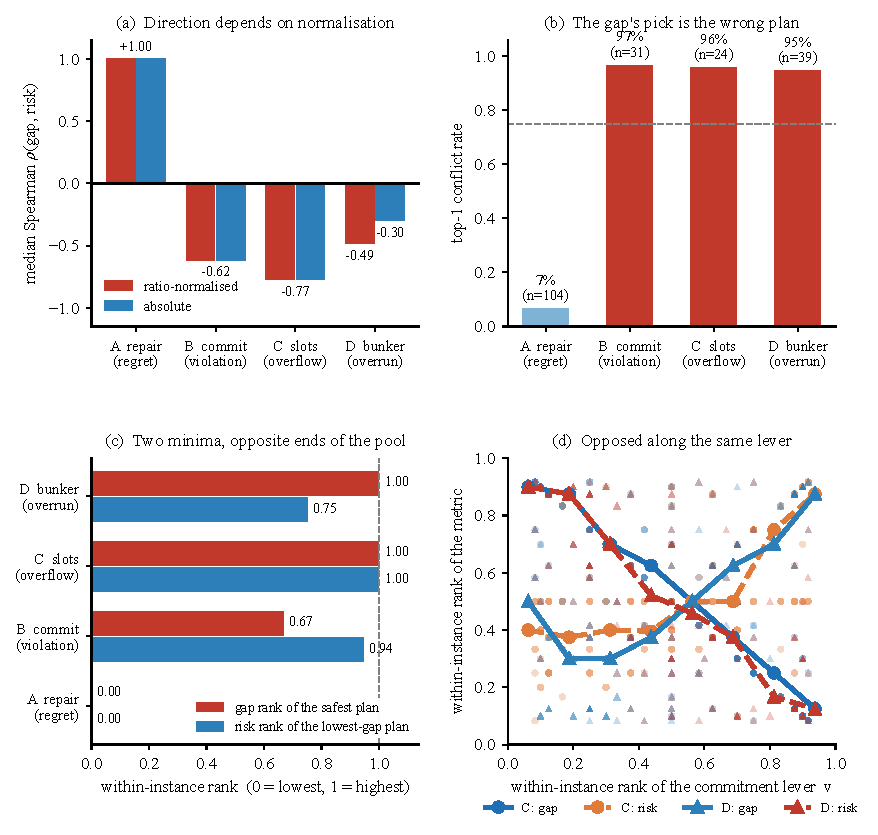
\includegraphics[width=\textwidth]{Figure_1.pdf}
\caption{Why an optimality gap is not a risk ordering. (a) Median within-instance Spearman correlation between the gap and the realised exposure, for the ratio-normalised and the absolute gap, in the four families; the sign of the association depends on the normalisation in D, and it is positive only in the repair regime A. (b) Top-1 conflict rate --- the share of instances in which the gap-minimal plan is not the exposure-minimal plan --- with the chance level for a four-candidate pool computed as $1 - 1/n$; A and B use the same candidate sets and differ only in whether the plan may be revised. (c) Positions of the two minima on a within-instance rank scale from 0 (bottom of the pool) to 1 (top): the gap rank of the safest plan and the risk rank of the gap-minimal plan. (d) The mechanism, on the same rank scale: the within-instance rank of the commitment lever $v$ against the within-instance rank of the gap (solid) and of the realised exposure (dashed), for C (lever = committed TEU) and D (lever = lift coverage), with binned medians overlaid. All panels are computed from the archived per-instance metrics of \S 9.}
\end{figure}
\clearpage

\begin{figure}[p]
\centering
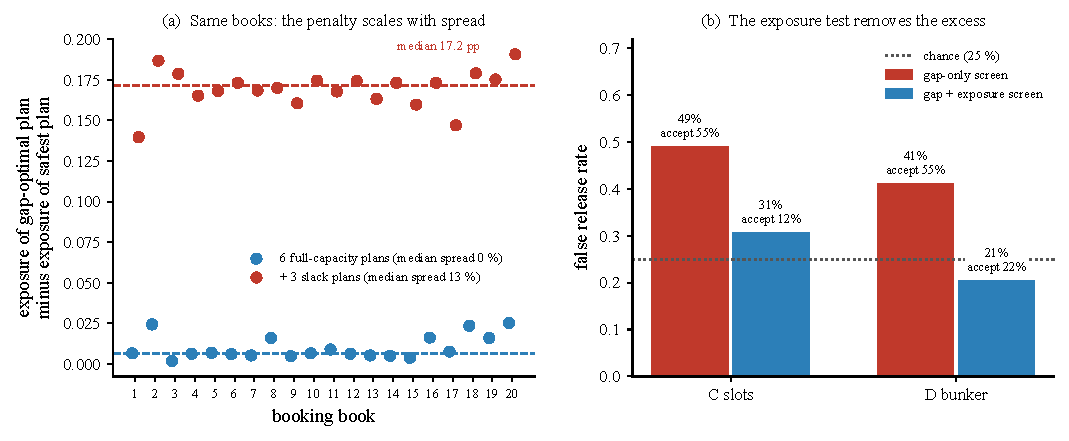
\includegraphics[width=\textwidth]{Figure_2.pdf}
\caption{The lever-spread manipulation and the two-dimensional release test. (a) For each of the twenty booking books, the realised exposure of the gap-minimal plan minus that of the exposure-minimal plan, in the two arms that differ only in the spread of committed volume: six full-capacity plans (median spread 0 \%) and the same six plus three deliberate-slack plans (median spread 13.2 \% of mean committed TEU); the dashed lines are the arm medians, 0.7 and 17.2 percentage points. (b) False-release rate of a gap-only screen and of a screen that adds an exposure quantile, at the operating threshold $\tau = 0.5$, with the corresponding acceptance rates printed above each bar, for families C and D under adverse drift. The 25 \% level a random release would produce is marked in panel (b).}
\end{figure}
\clearpage

\begin{figure}[p]
\centering
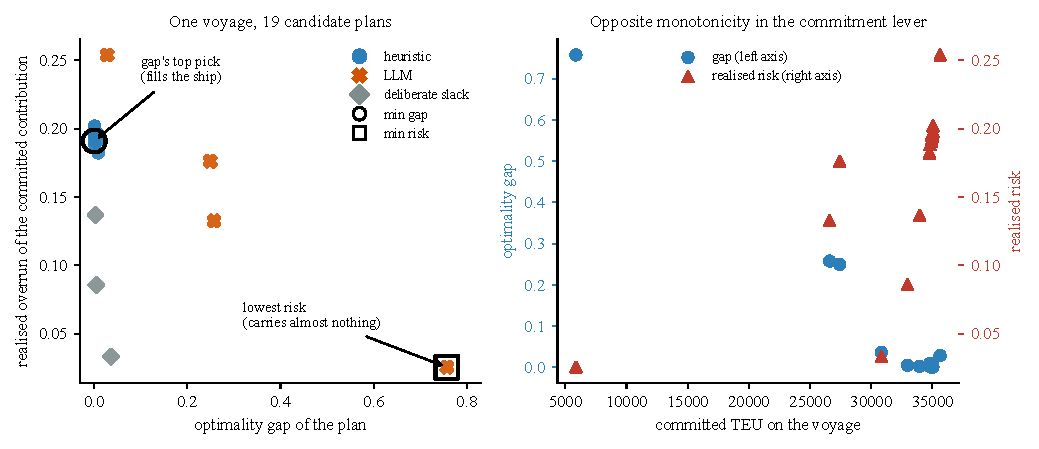
\includegraphics[width=\textwidth]{Figure_3.pdf}
\caption{One calibrated voyage. Left: the nineteen candidate plans in gap--exposure space, with the gap-minimal plan ringed by a circle and the exposure-minimal plan ringed by a square; markers distinguish heuristic, language-model and deliberate-slack plans. Right: the same plans against committed TEU, with the optimality gap on the left axis and the realised exposure on the right axis, showing the two moving in opposite directions along the commitment lever. The rotation, capacities, prices, tank limits and the mixed-integer program that generate the plans are given in \S 5.7 and \S 9.}
\end{figure}
\clearpage

\begin{figure}[p]
\centering
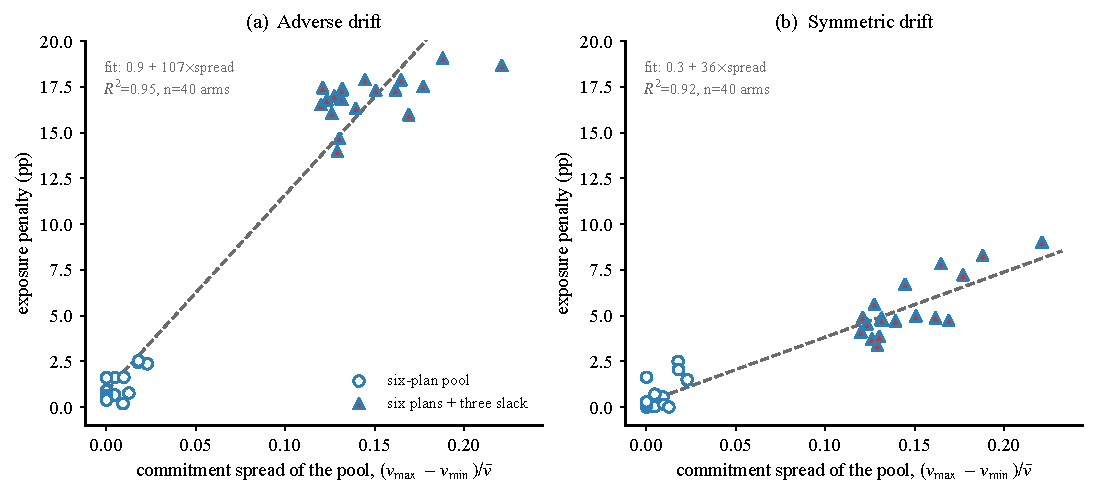
\includegraphics[width=\textwidth]{Figure_4.pdf}
\caption{The magnitude law of Corollary 1 on the twenty-book ensemble. Each point is one book under one arm under one drift direction, eighty observations in all: the commitment spread of the pool, $(\max - \min )/mean$ committed TEU, against the exposure penalty, the realised exposure of the gap-minimal plan minus that of the exposure-minimal plan. (a) Adverse drift: open circles are the six full-capacity plans, filled triangles the same six plus three deliberate-slack plans; the dashed line is the least-squares fit $0.9 + 107 \times spread$ ($R^{2} = 0.95$, forty arms). (b) Symmetric drift: $0.3 + 36 \times spread$ ($R^{2} = 0.92$). The slope is the exposure slope of Corollary 1, and it is three times smaller under mean-zero drift. Data: \texttt{rev2b\_\allowbreak{}books\_\allowbreak{}arms.\allowbreak{}csv}.}
\end{figure}
\clearpage

\begin{figure}[p]
\centering
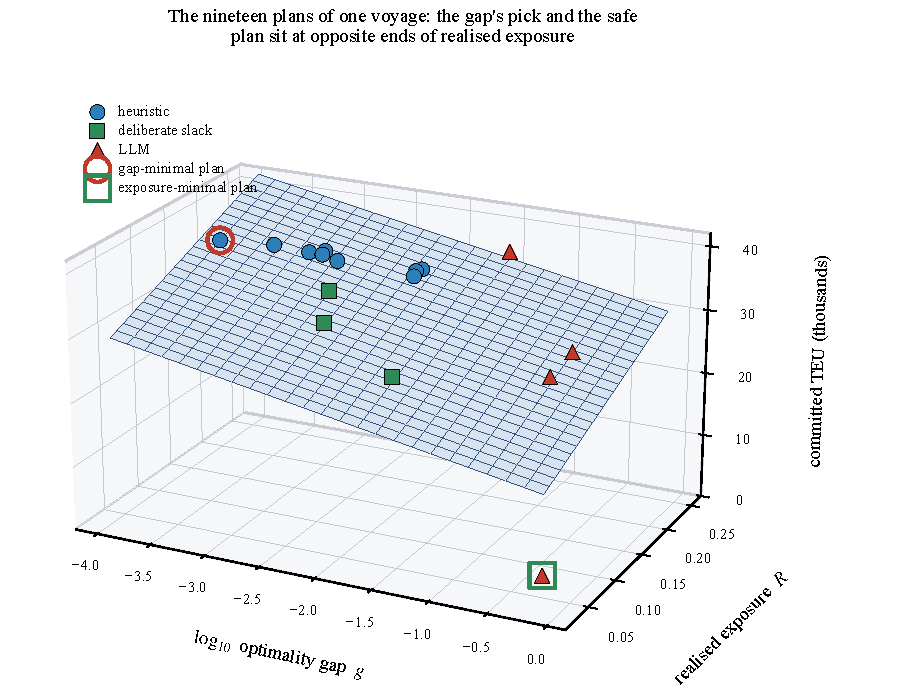
\includegraphics[width=\textwidth]{Figure_5.pdf}
\caption{The nineteen voyage plans of \S 5.7 in three dimensions: $\log_{10}$ optimality gap, realised exposure, and committed TEU in thousands. Blue circles are heuristic plans, green squares deliberate-slack plans and red triangles language-model plans; the ringed points are the gap-minimal and the exposure-minimal plan. The gap's pick sits at the low-gap, high-exposure, high-volume corner and the safe plan at the diagonally opposite corner, so the vertical axis is the lever along which the two minima separate. The pale gridded surface is the least-squares fit of committed volume on the two metrics, drawn only across the range the plans themselves span; it is a visual guide to the diagonal, not a model. This is the three-dimensional reading of Fig. 3. Data: \texttt{real\_\allowbreak{}case\_\allowbreak{}plans.\allowbreak{}csv}.}
\end{figure}
\clearpage

\begin{figure}[p]
\centering
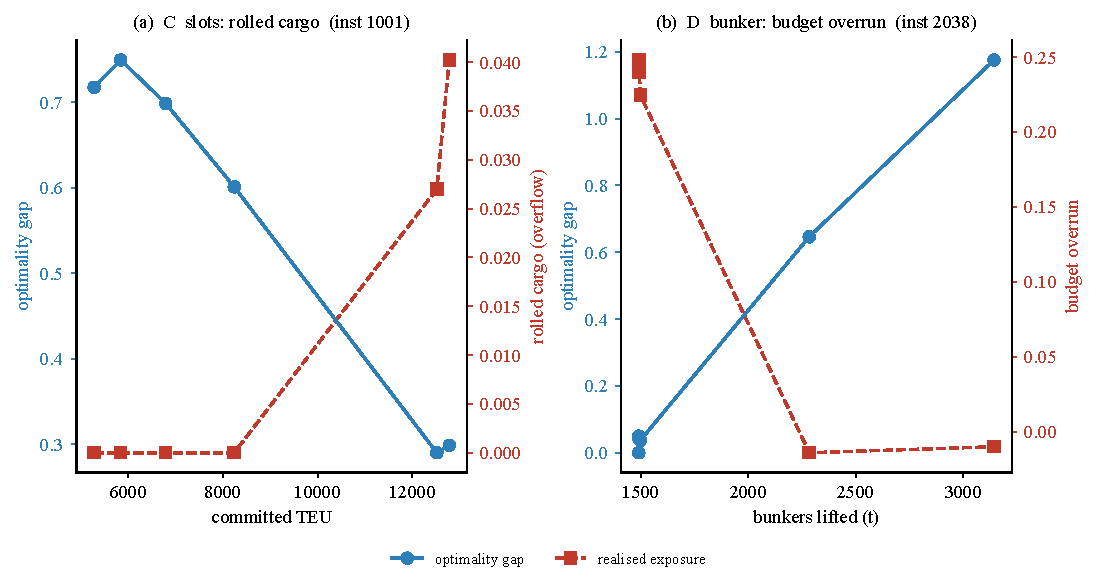
\includegraphics[width=\textwidth]{Figure_6.pdf}
\caption{The lever mechanism in one instance per family. The instance plotted is the one whose within-instance rank correlation between gap and exposure is closest to the family median (C, $-$0.775; D, $-$0.486), restricted to pools of at least five plans in which both quantities take three or more distinct values; it is the median instance, not the most favourable one. (a) C slots, instance 1001: optimality gap (left axis, blue) and rolled cargo (right axis, red) against committed TEU. (b) D bunker, instance 2038: gap (left) and budget overrun (right) against lifted tonnes. The two axes are read independently; what the panels show is one quantity falling while the other rises along the same decision variable. Data: \texttt{llm\_\allowbreak{}slot\_\allowbreak{}candidates.\allowbreak{}csv}, \texttt{llm\_\allowbreak{}bunker\_\allowbreak{}candidates.\allowbreak{}csv}.}
\end{figure}
\clearpage

\begin{figure}[p]
\centering
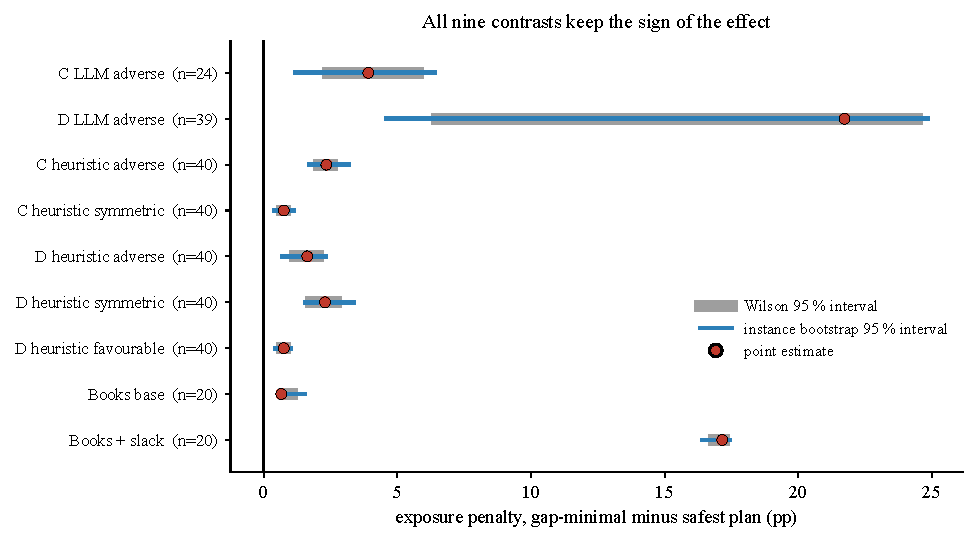
\includegraphics[width=\textwidth]{Figure_7.pdf}
\caption{The nine paired contrasts of Table 4. For each row, the exposure penalty of the gap-minimal plan over the exposure-minimal plan in percentage points, with the Wilson interval of the binomial read (thick grey), the 5,000-resample instance bootstrap interval (blue), both at 95 \%, and the point estimate in red. The vertical line is zero; every interval lies on one side of it, and all do so after a Bonferroni correction for nine comparisons. The width of each interval is the precision with which that row's magnitude is known. Data: \texttt{effect\_\allowbreak{}ci.\allowbreak{}csv}.}
\end{figure}
\clearpage

\begin{figure}[p]
\centering
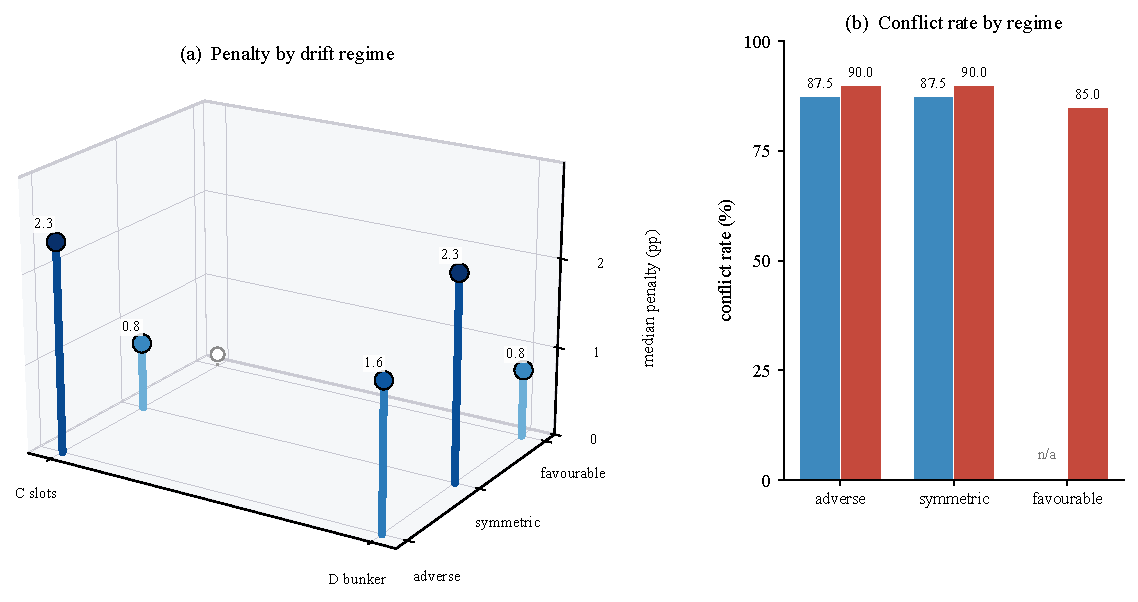
\includegraphics[width=\textwidth]{Figure_8.pdf}
\caption{Drift direction against family. (a) Median exposure penalty in percentage points on the family $\times$ regime grid, drawn as stems from the zero plane and shaded by magnitude, with the value printed at each stem head; the open circle marks C under favourable drift, where no plan overflows and no instance is usable. (b) Top-1 conflict rate by drift regime, C in blue and D in red; the absent blue bar at favourable drift is the same empty cell. The conflict rate is nearly flat across drift while the penalty is not, which is the reading of \S 5.4. Data: \texttt{rev2\_\allowbreak{}drift.\allowbreak{}csv}, forty instances per family and regime.}
\end{figure}
\clearpage

\begin{figure}[p]
\centering
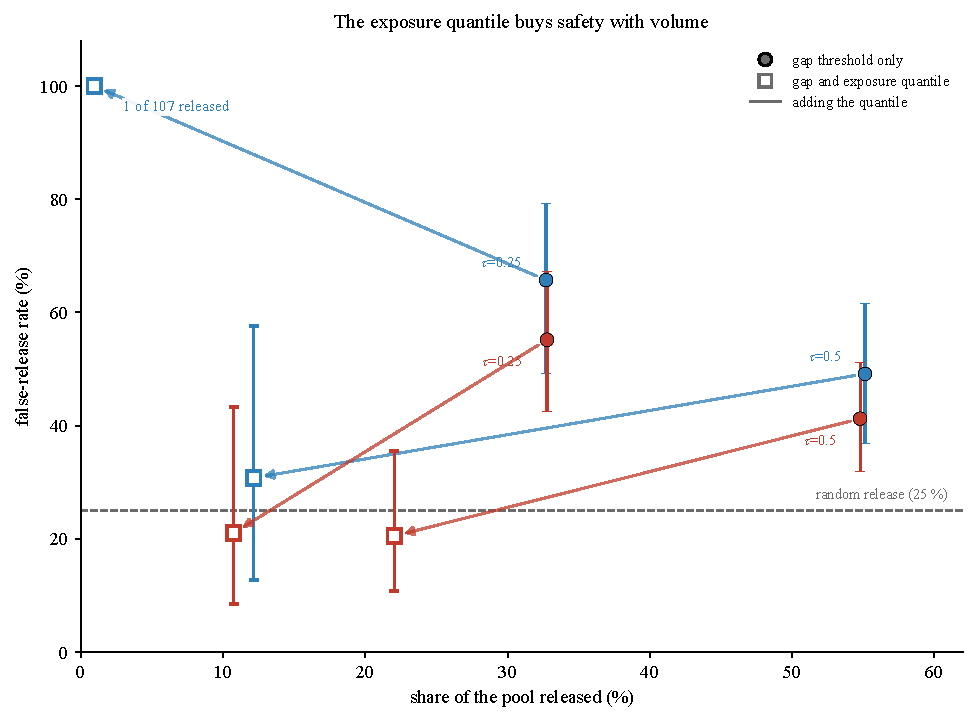
\includegraphics[width=\textwidth]{Figure_9.pdf}
\caption{Release-rule operating points for the four cells of Table 6: the share of the candidate pool released against the false-release rate. Filled circles screen on the gap alone, open squares add the exposure quantile, and the arrow connects the two at fixed $\tau$ and family. Error bars are Wilson 95 \% intervals; the point at the top left is 1 of 107 released, whose rate is not estimated. The dashed line is the 25 \% a random release would produce --- the benchmark, not zero. Data: \texttt{screen\_\allowbreak{}ci.\allowbreak{}csv}.}
\end{figure}
\clearpage

\begin{figure}[p]
\centering
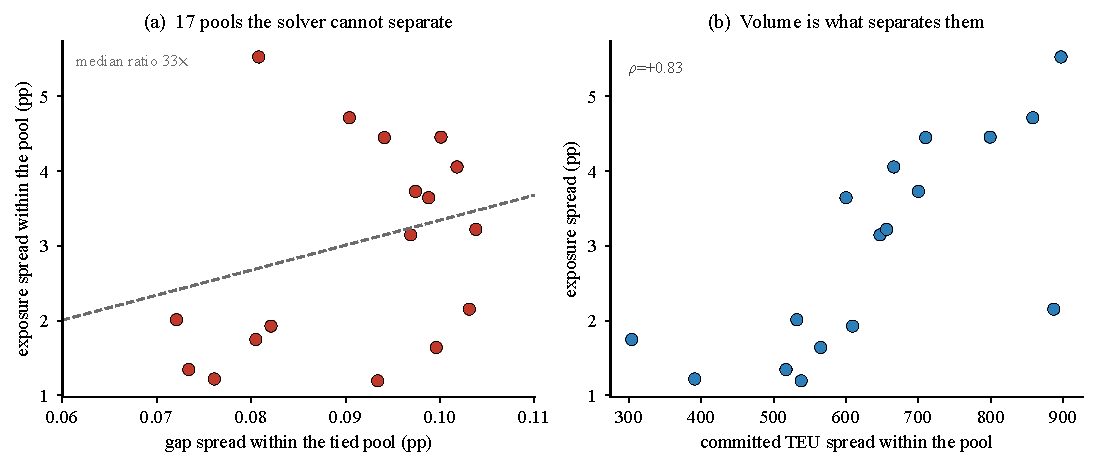
\includegraphics[width=\textwidth]{Figure_10.pdf}
\caption{The resolution limit inside a tie. (a) For each of the seventeen booking books that admit a tied pool of at least five plans, the gap spread within the pool against the exposure spread; the dashed line is the median ratio, 33 times. (b) The same exposure spread against the committed-volume spread ($\rho = 0.83$). Every pool lies far above the one-to-one line of panel (a), so the exposure variation the certificate cannot see is never a small multiple of the variation it can. Data: \texttt{tie\_\allowbreak{}pool.\allowbreak{}csv}.}
\end{figure}
\clearpage

\end{document}
